\documentclass[Thesis]{subfiles}

\begin{document}

\newpage
\chapter{Location--Scale Models in Demography: A Useful Re-parameterization of Mortality Models}\label{Ch2}\chaptermark{Location--scale models in demography}
\thispagestyle{empty}
\pagecolor{pagecolor}\afterpage{\nopagecolor}
\vspace{1cm}
\Large
Ugofilippo Basellini\\
Vladimir Canudas-Romo\\
Adam Lenart 
\vspace{2cm}
\textit{\\ European Journal of Population}, \textbf{35}(4), 645--673 (2019). \\
DOI: \href{https://link.springer.com/article/10.1007/s10680-018-9497-x}{\color{black}10.1007/s10680-018-9497-x}
\clearpage

\thispagestyle{empty}
\pagecolor{pagecolor}\afterpage{\nopagecolor}
\section*{}
\clearpage


% % --------------------------------------------

\thispagestyle{empty}
{\centering
{\Large\bfseries Location--Scale Models in Demography: A Useful Re-parameterization of Mortality Models \par}
\vspace{0.5cm}
{\large Ugofilippo Basellini$^{1,2,\dagger}$, Vladimir Canudas-Romo$^{3}$, and Adam Lenart$^{2}$  \par}
\singlespacing
{\normalsize $^{1}$\itshape Institut national d'\'{e}tudes d\'emographiques (INED), Paris, France\\[2mm]}
{\normalsize  $^{2}$\itshape Interdisciplinary Centre on Population Dynamics (CPop) and Department of Public Health, University of Southern Denmark, Odense, Denmark\\[2mm]}
{\normalsize $^{3}$\itshape School of Demography, Australian National University, Canberra, Australia\\[2mm]}
{\normalsize $^{\dagger}${\itshape Corresponding author:} \url{ugofilippo.basellini@ined.fr}\\
\vspace{0.5cm} This is a post-peer-review, pre-copyedit version of an article published in \\ \textit{European Journal of Population}. The final authenticated version is available online at: \url{https://link.springer.com/article/10.1007/s10680-018-9497-x} \\  
\vspace{0.5cm} Submitted: December 2017; Accepted: September 2018	 \par}
\vspace{1.0cm}
{\bfseries Abstract \\[5mm]}
\onehalfspacing
{\normalsize \justify Several parametric mortality models have been proposed to describe the age pattern of mortality since Gompertz introduced his "law of mortality" almost two centuries ago. However, very few attempts have been made to reconcile most of these models within a single framework. In this article, we show that many mortality models used in the demographic and actuarial literature can be re-parameterized in terms of a general and flexible family of models, the family of location--scale (LS) models. These models are characterized by two parameters that have a direct demographic interpretation: the location and scale parameters, which capture the shifting and compression dynamics of mortality changes, respectively. Re-parameterizing a model in terms of the LS family has several advantages over its classic formulation. In addition to aiding parameter interpretability and comparability, the statistical estimation of the LS parameters is facilitated due to their significantly lower correlation. The latter, in turn, further improves parameter interpretability and reduces estimation bias. We show the advantages of the LS family over the typical parameterization of mortality models with two illustrations using the Human Mortality Database. \par 
\vspace{0.5cm}	
\noindent \textbf{Keywords:} Mortality Modelling$\;\cdot\;$Law of Mortality$\;\cdot\;$Shifting$\;\cdot\;$Compression$\;\cdot\;$Gamma-Gompertz$\;\cdot\;$\\Extreme-Value}
}

\newpage

% --------------------------------------------

\normalsize

\section{Introduction}
\label{Sec:Ch2sec1}

\subsection{Parametric mortality models}
\label{Subsec:Ch2subsec1.1}

The search for a model of human mortality has a fairly long history: mortality modelling has indeed developed into an established research topic since the first half of the eighteenth century \citep{tabeau2001review}. In particular, several efforts have been directed towards parametric models, which assume a parametric distribution to describe the age pattern of mortality.

Parametric models have long been used by actuaries, demographers and medical scientists for smoothing data, eliminating and/or reducing errors, constructing life tables, aiding inferences from incomplete data, facilitating comparisons of mortality, and forecasting \citep{keyfitz1982choice}. The popularity of these models can be attributed to at least six advantages of representing mortality schedules with a single curve governing all data points \citep{congdon1993statistical}: 
\begin{enumerate}
	\item[(a)] \textit{Smoothness}: there are no uneven age-variations of mortality rates due to random statistical fluctuations. This is particularly advantageous when looking at very old-age mortality, where the number of deaths and exposure-to-risk are much smaller than at other ages.
	\item[(b)] \textit{Parsimony}: mortality schedules of several points corresponding to many different ages can be represented only by a few parameters. 
	\item[(c)] \textit{Interpolation}: mortality rates for any specific age can be analytically derived. In practice, this is very important when only five-year age-group rates are known, or when the mortality schedule is incomplete.
	\item[(d)] \textit{Comparison}: mortality data always refer to a specific population, which could be as broad as the national population of a country, or as narrow as the policyholders of an insurance company. Populations differ by their composition of gender, age, marital and social status, lifestyle, health and regional geography (e.g. postcode). The comparison of several mortality patterns can be readily and more easily performed by estimating the model's parameters for each population studied.
	\item[(e)] \textit{Trends and forecasting}: the assessment of trends over time and forecasting into the future are facilitated.
	\item[(f)] \textit{Analytic manipulation}: the properties of the model employed are generally known, and these can be used in more complex demographic settings. For example, one common procedure is to specify the uncertainty associated with the model projections. 
\end{enumerate}

More recently, parametric models have been used to study the shifting and compression dynamics of mortality changes. The remarkable mortality reductions that occurred in most developed countries during the twentieth century are generally divided into two different stages. In the first half of the century, fast mortality declines at younger ages produced a compression of the age-at-death distribution, with the majority of deaths concentrated in a smaller age-interval  \citep{fries1980aging,myers1984compression,rothenberg1991population,kannisto2000measuring,cheung2009dissecting}. Then, as rates of mortality improvements slowed down at younger ages and accelerated at older ages \citep{kannisto1994reductions,vaupel1998biodemographic,wilmoth1999rectangularization}, the distribution of deaths started to shift to older ages, with a shape remaining practically constant \citep{bongaarts2005long,cheung2005three,cheung2007increase,canudas2008modal}.

\cite{bergeron2015decomposing} introduced a decomposition method based on a re-parameterization of mortality models that allows to differentiate between the two dynamics and estimate their contribution to increases in life expectancy. In particular, the authors find that the shifting dynamic was responsible for more than 70\% of the increase in average lifespan for Swedish females since the mid-1960s. Furthermore, \cite{de2016new} presented a new parametric model that formally captures the two dynamics, and they show that two-thirds of the increases in life expectancy for Japanese, French, American and Danish females and males between 1950 and 2010 were due to shifting mortality.

\subsection{Short history of parametric mortality models}
\label{Subsec:Ch2subsec1.2}

The research of a "law of mortality" has been an interesting topic since the development of the first life tables by \cite{graunt1662natural} and \cite{halley1693estimate}. One of the very first attempts to model mortality with a parametric distribution goes back to \cite{demoivre1725annuities}. A century later, \cite{gompertz1825nature} made one of the most well-known early contributions to the field, as he theorized an increasing exponential effect of age on the force of mortality. 

A few years later, \cite{makeham1860law} suggested a modification of the Gompertz model to overcome the underestimation of mortality at young adult ages by adding a constant non-ageing-related risk term. Shortly afterwards, \cite{thiele1871mathematical} proposed a model to capture the non-monotonic shape of human mortality along the full age range. In particular, he suggested to decompose human mortality into three different groups that operate principally, or almost exclusively, upon childhood, middle and old ages, respectively. This assumption has been extensively used since then for modelling purposes \citep{siler1979competing,heligman1980age}. 

The Logistic model, first discovered by \cite{perks1932some}, is a general model which includes the Makeham law as a special case. Recently, this model has been used to describe the force of mortality at very high ages, for example above age 80 \citep{wilmoth2000increase}: the logistic function implies that death rates approach a fixed upper limit, as suggested both empirically and theoretically \citep{vaupel1998biodemographic, gampe2010human}. 

Subsequently, the Gamma-Makeham model was introduced by \cite{beard1971some}, who showed that a logistic function could arise in a simple model of a heterogeneous population. Indeed, the aggregation of several individual Makeham hazards with different levels of initial mortality can result in a logistic curve \citep{thatcher1998force}. Afterwards, this finding was developed extensively as the \emph{frailty} model \citep{vaupel1979impact}.  

Along with the Gompertz, the Weibull model is widely used as a parametric form of the hazard function to adequately capture the ageing process \citep{missov2015mortality}. \cite{weibull1951statistical} introduced this model to represent the durability and failure due to wear and tear of technical systems, such as ball bearings, automobile components, and electrical insulation. An analogy to mortality can be made by considering death as the result of the failure of bodily organs or damage to cells \citep{thatcher1998force}. The model has been used extensively in biological and medical research, for example, in studies on the time of occurrence of tumours in human populations or laboratory animals \citep{lawless2011statistical}. 

One limitation of all the models for adult mortality  mentioned above is that their hazard function, be it  increasing, decreasing or constant, must be monotonic, whatever the values of the parameters. This may be inappropriate in some settings, for example when the course of a disease is such that mortality reaches a peak after some finite period, and then slowly declines. Among others, two models have been proposed to overcome this issue: the Log-Logistic and the Log-Normal models. Indeed, these models have non-monotonic hazard functions, which make them suitable in several situations, such as the modelling of some sets of cancer survival data \citep{bennett1983log}.

Finally, in recent years, it has been claimed that the Extreme-Value model could provide great future prospects for mortality analysis and forecasting \citep{willekens2001gompertz}. This model is generally used to describe the failure times or lifetimes of systems that cease to function whenever the weakest component fails. 

\subsection{Aims}
\label{Subsec:Ch2subsec1.3}

In this paper, we aim to show that several well-known mortality models can be re-parameterized in terms of two parameters that describe the shifting and compression dynamics of mortality changes. These models belong to a rather general family of parametric models, the family of location--scale (LS) models. The parameters of the LS family have a direct demographic interpretation, and as such, they are easier to understand than those of the classic formulation of mortality models.

In addition, re-parameterizing mortality models in terms of the LS family has an important statistical advantage: the estimation of the LS parameters is greatly facilitated, as the rather high correlation between estimators of the classic models is significantly reduced. The lower correlation, in turn, improves parameter interpretability and reduces estimation bias.

This article is organized as follows. In Section \ref{Sec:Ch2sec2}, we provide an overview of the mathematical methods that we use throughout this article. In particular, we first present the family of LS models, and we show that several parametric models belong to the family. In addition, we describe the data that we employ in this article, and the estimation procedure for the models' parameters. In Section \ref{Sec:Ch2sec3}, we present two illustrations that demonstrate the advantages of the LS family over the classic parameterization of mortality models. First, we assess the shifting and compression dynamics of mortality changes directly from the estimation of the LS parameters in four high-longevity countries during the years 1960-2016 by gender. Second, we show that the estimated parameters of the LS family have a significantly lower \textit{between} and \textit{within} country correlation than classic models for females and males in thirty-three countries from 1960 until the most recent available year. In Section \ref{Sec:Ch2sec4}, we discuss the results and we conclude.

\section{Methods}
\label{Sec:Ch2sec2}

\subsection{Life-table functions}
\label{Subsec:Ch2subsec2.1}
Let $l(x)$ be the life-table probability of surviving from birth to age $x$, and $\mu (x)$ be the force of mortality at age $x$. Then, we have that $l(x)=l(0)e^{- \int_{0}^{x} \mu (a)da}$, where $l(0)$ is the radix of the population. Moreover, let $f(x)$ be the probability density function describing the distribution of deaths in the life-table population at age $x$. Then, $\int_{0}^{\omega}f(a)da=l(0)$, where $\omega$ is the highest age attained in the population. For simplicity, we let $l(0)$ be equal to one. The relationship that exists between the distribution of deaths, the force of mortality and the survival function for a given age $x$ is $f(x)=\mu (x)l(x)$ \citep{preston2001demogr}.


\subsection{The location--scale family of mortality models}
\label{Subsec:Ch2subsec2.2}

Location--scale distributions are well-known in reliability theory and lifetime data analysis. As such, we define the location--scale (LS) family of mortality models according to the literature. Specifically, let $X$ be a continuous random variable. We say that $X$ belongs to the LS family if we can express the probability density function $f(x)$ as: 
\begin{eqnarray}\label{Eq:Ch2LSpdf}
f(x)= \frac{1}{c} \, f_{LS} \left (\frac{x-u}{c} \right ), \quad x\in\mathbb{R} \, ,
\end{eqnarray}
where $u \in \mathbb{R}$ and $c > 0 $ are the location and scale parameters respectively, and $f_{LS}(\cdot)$ is a continuous function that does not depend on any unknown parameters. In particular, $f_{LS}(\cdot)$ represents the standard form of the distribution, i.e.~when $u=0$ and $c=1$.

Similarly, we say that $X$ belongs to the log--location--scale (LLS) family of models if we can express the probability density function $f(x)$ as: 
\begin{eqnarray}\label{Eq:Ch2LSLpdf}
f(x)=\frac{1}{c\,x} \, f_{LLS} \left (\frac{\ln(x)-u}{c} \right ),  \quad x>0 \, ,
\end{eqnarray}
where the parameters $u$, $c$ and $f_{LLS}(\cdot)$ are defined as in equation (\ref{Eq:Ch2LSpdf}) \citep{mukhopadhyay2000probability,lawless2011statistical,meeker2014statistical}.

Equivalently, the two families can be defined in terms of the force of mortality $\mu(x)$. Specifically, for the LS family the force of mortality satisfies:
\begin{eqnarray}\label{LSMmux}
\mu(x)= \frac{1}{c} \, \mu_{LS} \left (\frac{x-u}{c} \right ), \quad x\in\mathbb{R} \, ,
\end{eqnarray}
while for the LLS family $\mu(x)$ satisfies:
\begin{eqnarray}\label{LSLMmux}
\mu(x)=\frac{1}{c\,x} \, \mu_{LLS} \left (\frac{\ln(x)-u}{c} \right ),  \quad x > 0 \, ,
\end{eqnarray}
where $u$ and $c$ are defined as above, and $\mu_{LS}(\cdot)$ and $\mu_{LLS}(\cdot)$ represent the standard form of the force of mortality (i.e.~when $u=0$ and $c=1$) for the two families, respectively.

The role of the location and scale parameters can be easily understood with an illustration. Figure \ref{Fig:Ch2locscalepdf} shows the effects of changes in the two parameters on the density function of the LS family of mortality models. 

\begin{figure}[!ht]
	\centering
	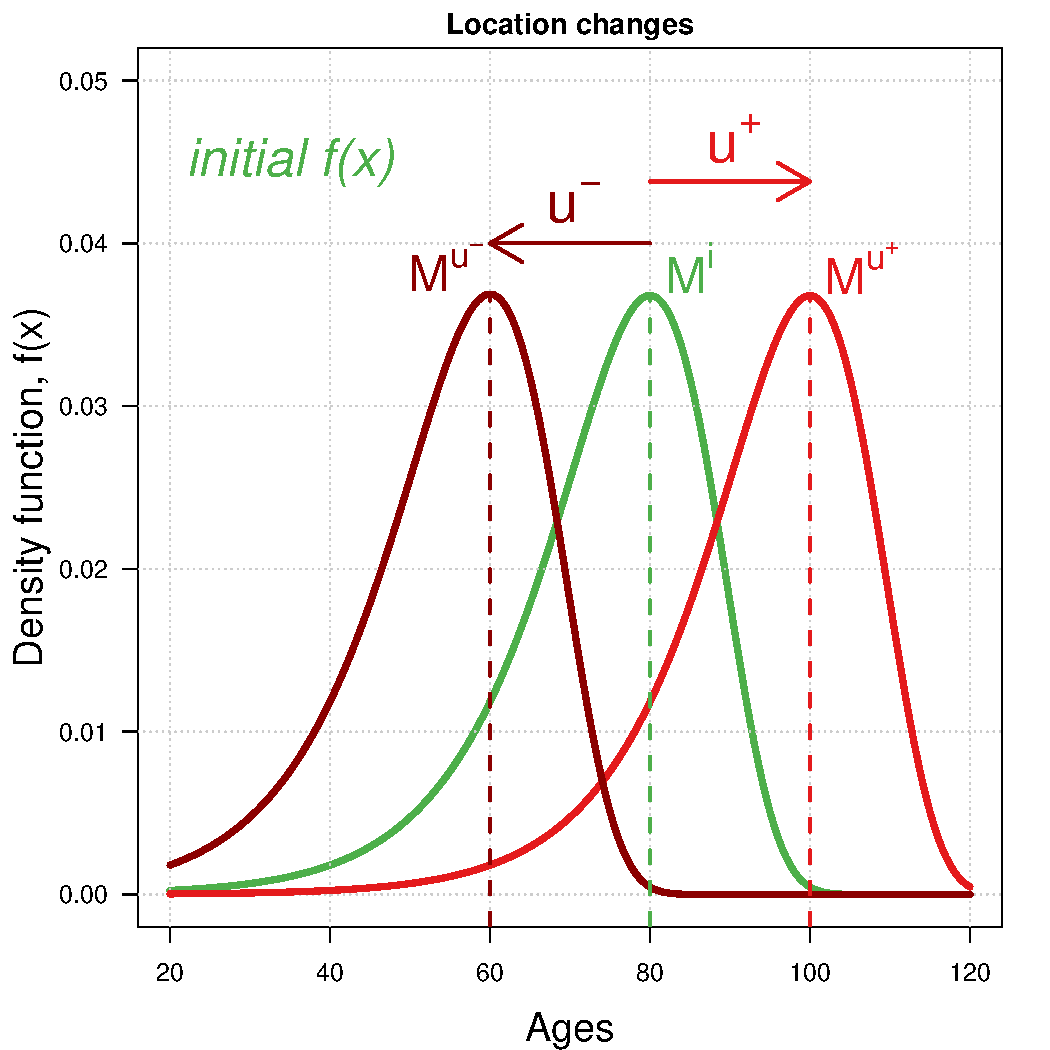
\includegraphics[scale=0.4]{./Ch2/F1a.pdf}
	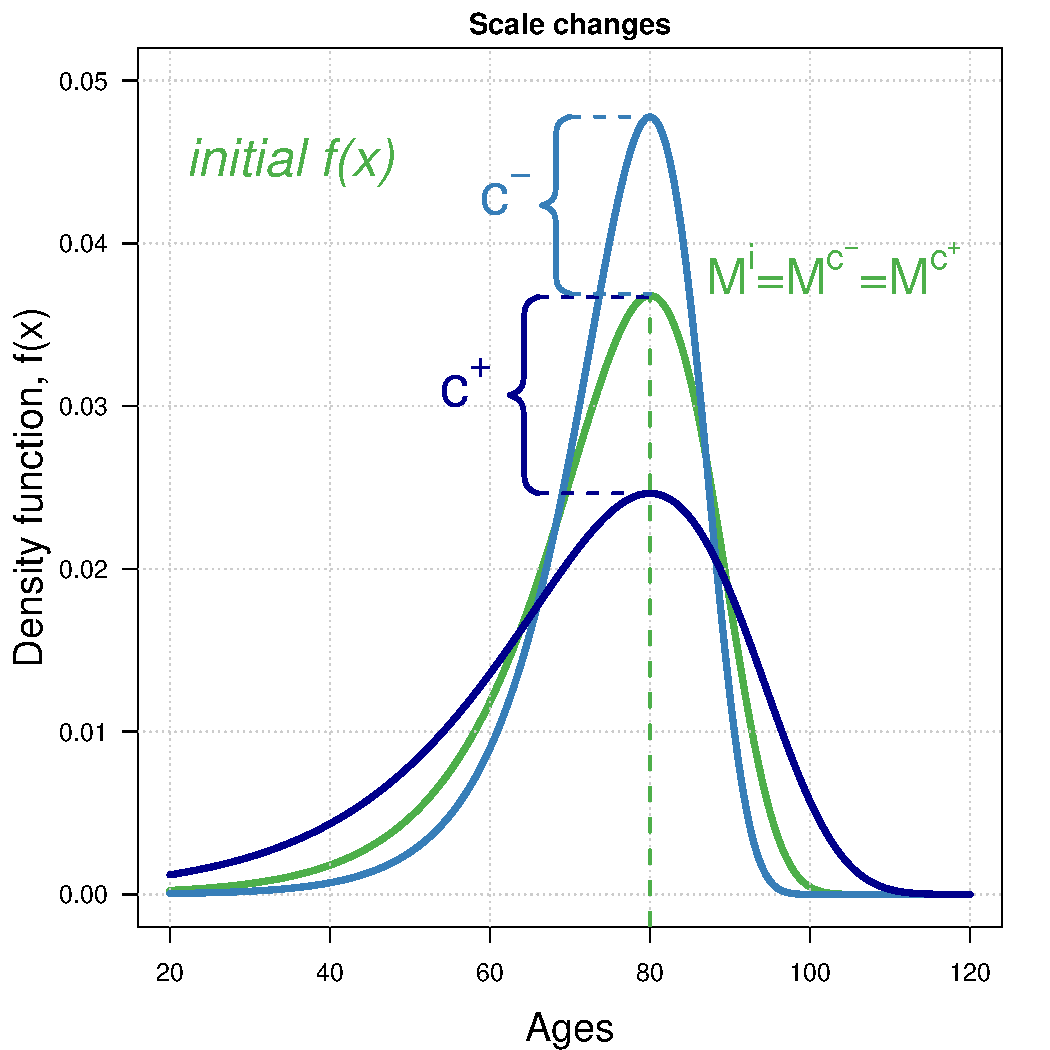
\includegraphics[scale=0.4]{./Ch2/F1b.pdf}
	
	\caption{Illustration of changes in the location $u$ (left panel) and scale $c$ (right panel) parameters on the density function $f(x)$ of the location--scale family of mortality models. The density corresponds to the Gompertz model, and changes for $u$ are from 80 to 60 ($u^-$) and 100 ($u^+$), and for $c$ from 10 to 7.7 ($c^-$) and 15 ($c^+$). $M$ denotes the old-age modal age at death.\\ \textit{Source (Figs.~\ref{Fig:Ch2locscalepdf}-\ref{Fig:Ch2locscaleMU}): Authors' own elaborations.}}\label{Fig:Ch2locscalepdf}

\end{figure}

The location parameter $u$ shifts the density function $f(x)$ along the $x$-axis without altering its shape. In the left panel of Figure \ref{Fig:Ch2locscalepdf}, an increase (decrease) in $u$ shifts the initial density to the right (left): this effect can be interpreted as a postponement (anticipation) of mortality. As such, changes in the parameter $u$ correspond to a pure \textit{shifting} effect, that is a shift of the density to older (younger) ages, without any shape changes.

The scale parameter $c$ affects the variability of the density function. In the right panel of Figure \ref{Fig:Ch2locscalepdf}, a decrease (increase) in $c$ results in a compression (expansion) of the initial density around the  old-age modal age at death $M$ (the adult age at which most of the deaths occur). As such, changes in the parameter $c$ correspond to a pure \textit{compression} effect. 

Figure \ref{Fig:Ch2locscaleMU} shows the corresponding effects of these changes on the force of mortality $\mu(x)$. In the left panel, location changes correspond to shifts of the mortality pattern (which are parallel for the Gompertz case shown in the Figure); increases in $u$ move $\mu(x)$ to the right (or down), while decreases in $u$ result in left (or upwards) shifts. In the right panel, changes in the scale parameter modify the slope of the mortality pattern. This effect can be interpreted as a change in the "speed" of mortality: a decrease (increase) in $c$ accelerates (slows down) the ageing process, so that mortality increases at a faster (lower) rate.

\begin{figure}[!ht]
	\centering
	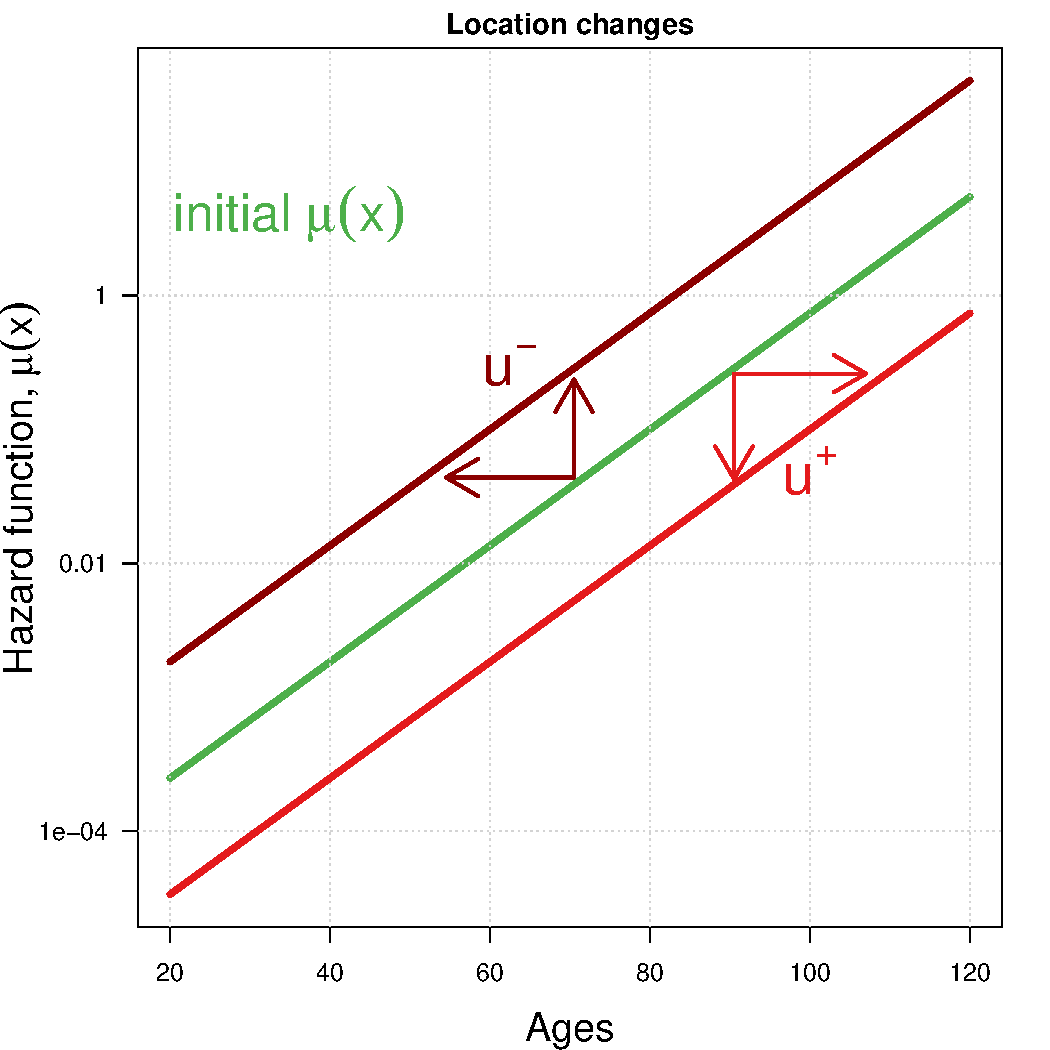
\includegraphics[scale=0.4]{./Ch2/F2a.pdf}
	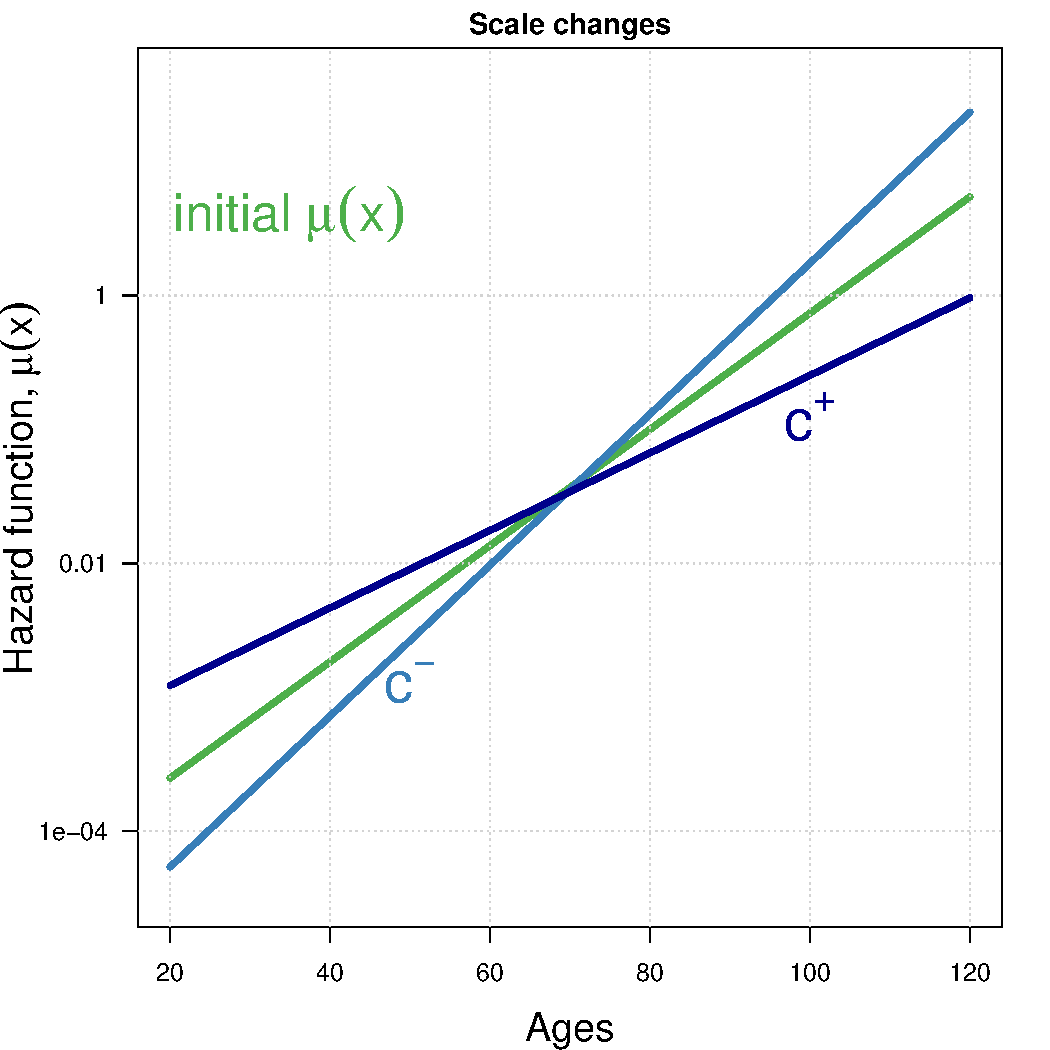
\includegraphics[scale=0.4]{./Ch2/F2b.pdf}
	
	\caption{Illustration of changes in the location $u$ (left panel) and scale $c$ (right panel) parameters on the force of mortality $\mu(x)$ (in log scale) of the location--scale family of mortality models. The force of mortality corresponds to the Gompertz model, and changes for $u$ and $c$ are the same as in Fig.~\ref{Fig:Ch2locscalepdf}.}\label{Fig:Ch2locscaleMU}
	
\end{figure}

The location and scale parameters thus capture and disentangle the shifting and compression dynamics of mortality. While we have shown the two effects in isolation for illustrative purposes, mortality changes typically occur simultaneously, and the two parameters can vary at the same time.

We can now proceed to show that several mortality models used in the demographic and actuarial literature belong to the LS family of mortality models. We first show this with a detailed derivation for the Gompertz model in the next Section (and for the Weibull model in Appendix \ref{Subsec:Ch2appA}). Then, we present a summary Table of the mortality models that can be reconciled with the LS family in Section \ref{Subsec:Ch2subsec2.4}.

\subsection{Gompertz and the location--scale family}
\label{Subsec:Ch2subsec2.3}

A model that is often used in demographic and actuarial analysis is the Gompertz model. This is one of the earliest attempts to find a "law of mortality": at the beginning of the nineteenth century, \cite{gompertz1825nature} discovered that for a large part of the age range (though not including infancy and youth or very old ages) the force of mortality increases with age at a steady exponential rate. The Gompertz model is generally expressed in the form:
\begin{eqnarray}\label{GompertzMu}
\mu (x)=ae^{bx} \, , \quad x \geq 0  \, ,
\end{eqnarray}
where $a > 0$ denotes the level of the force of mortality at the starting age of the analysis, and $b$ corresponds to the rate of ageing \citep{thatcher1998force}. From the life-table functions introduced in Section \ref{Subsec:Ch2subsec2.1}, we can derive the density function $f(x)$ of the Gompertz model:
\begin{eqnarray}\label{GompertzDens}
f(x) = \mu (x)l(x) = \mu (x) e^{- \int_{0}^{x} \mu (a)da}  = a \, \mathrm{exp} \left [ bx -\frac{a}{b} (e^{bx}-1) \right ] .
\end{eqnarray}

It is possible to show that the Gompertz model is closely related to the location--scale (LS) family of mortality models. In particular, the LS-like parameterization of the Gompertz model for the force of mortality is: 
\begin{eqnarray}\label{GompertzMuLS}
\mu(x) = \frac{1}{c} \, e^{\frac{x-u}{c}} \, , \quad x \geq 0 \, ,  
\end{eqnarray}
where $u \in \mathbb{R}$ and $c > 0$ are the location and scale parameters, respectively. The corresponding LS-like density function of the Gompertz model can be expressed as:
\begin{eqnarray}\label{GompertzDensLS}
f(x) = \frac{1}{c}\,\mathrm{exp} \left [ \frac{x-u}{c} - \mathrm{exp} \left ( \frac{x-u}{c} \right ) + \mathrm{exp} \left ( - \frac{u}{c} \right ) \right ]   \, .
\end{eqnarray}

Indeed, if we let the location and scale parameters be $u =  \frac{1}{b} \mathrm{ln} \left ( \frac{b}{a} \right )$ and $c=\frac{1}{b}$, and we substitute them in Equations (\ref{GompertzMuLS}) and (\ref{GompertzDensLS}), we obtain the classic Gompertz formulas in Equation (\ref{GompertzMu}) and (\ref{GompertzDens}). 

The Gompertz model does not strictly belong to the LS family of mortality models: its force of mortality is only defined for $x\geq0$, while the location--scale $\mu(x)$ can vary on the entire set $\mathbb{R}$ (see Equation (\ref{LSMmux})). The truncation of the $x$-axis can be also observed in the functional form of $f(x)$ in Equation (\ref{GompertzDensLS}), which depends on the parameters $u$ and $c$ via the $\mathrm{exp} \left ( e^{- \frac{u}{c}} \right )$ term. Nevertheless, the Gompertz model is closely related to a location--scale distribution, the Gumbel \cite[or type 1 extreme value distribution,][]{johnson1995continuous} : "\textit{the Gompertz distribution is a special case of the Gumbel distribution for the minima, i.e., when $x:=-x$ and truncated at $x=0$}" \cite[p.~2923,][]{lenart2016goodness}. As such, the Gompertz model can be considered a \textit{truncated} location--scale distribution.

The location and scale parameters of the Gompertz model are reported in Table \ref{Tab:Ch2LS} of the following Section, together with the formulas of the classic and LS-like $\mu(x)$; the classic and LS-like functional forms of $f(x)$ are reported in Table \ref{Tab:Ch2LSfx} of Appendix \ref{Subsec:Ch2appB}.

Finally, it is interesting to observe that, if we let the location parameter be equal to the old-age modal age at death $M$, that is $u=M$, and we keep $c=\frac{1}{b}$, then Equation (\ref{GompertzMuLS}) becomes:
\begin{eqnarray}\label{GompertzMuM}
\mu (x) = be^{b(x-M)} \, ,
\end{eqnarray}
which is the parameterization of the Gompertz model in terms of the modal age at death \citep{horiuchi2013modal, missov2015gompertz}.

\subsection{Other parametric mortality models}
\label{Subsec:Ch2subsec2.4}

Several models have been proposed to describe the age pattern of the force of mortality during the last two centuries \citep[for a comprehensive review, see][]{tabeau2001review}, and many of them can be unified under the overarching family of location--scale models. Table~\ref{Tab:Ch2LS} presents twelve well-known models of mortality that either belong to the location--scale (LS) and log-location--scale (LLS) families or that are closely related to them. The Table reports each model's parameterization in terms of the classic and LS force of mortality $\mu(x)$, $\mu_{LS}(x)$ or $\mu_{LLS}(x)$, location $u$ and scale $c$ parameters. The classic and LS functional form $f(x)$, $f_{LS}(x)$ or $f_{LLS}(x)$ are reported in the Table \ref{Tab:Ch2LSfx} in Appendix \ref{Subsec:Ch2appB}.

%\begin{landscape}
\begin{table}[!ht]
	\begin{center}
		\caption{Mortality models belonging to the location--scale (LS) and log--location--scale (LLS) families, and models closely related to them, together with their parameterization in terms of the classic, LS and LLS force of mortality $\mu(x)$, $\mu_{LS}(x)$, $\mu_{LLS}(x)$, location $u$ and scale $c$ parameters.}\label{Tab:Ch2LS}
		
		\scriptsize
		\begin{tabular}{l c c c c}						
			\\
			\toprule
			
			\begin{tabular}[c]{@{}l@{}}\textbf{Models belonging}\\ \textbf{to the LS family}\end{tabular} & $\qquad$ $\boldsymbol{\mu(x)}$ $\qquad$ &    $\boldsymbol{\frac{1}{c} \, \mu_{LS} \left (\frac{x-u}{c} \right )}$ & $\qquad$ $\boldsymbol{u}$ $\qquad$  & $\qquad$ $\boldsymbol{c}$ $\qquad$        \\	
			\midrule	 \\
			
			Logistic  & $\frac{b \, \mathrm{exp}(a+bx)}{1+ \mathrm{exp}(a+bx) }$ & $\frac{1}{c} \, \frac{\mathrm{exp}(\frac{x-u}{c})}{1+ \, \mathrm{exp}(\frac{x-u}{c})}$   & $ - \frac{a}{b} $ & $\frac{1}{b}$   \\ \\  \rowcolor{my-grey}
			
			Normal  & $ \frac{1}{\sigma} \, \frac{\phi \left ( \frac{x-\lambda}{\sigma}\right )}{ 1-\Phi \left ( \frac{x-\lambda}{\sigma}\right )} $ & $\frac{1}{c} \, \frac{\phi \left ( \frac{x-u}{c}\right )}{ 1-\Phi \left ( \frac{x-u}{c}\right )} $  & $\lambda $   &    $\sigma $         \\ \\		
			
			\begin{tabular}[c]{@{}l@{}}Smallest\\ Extreme-Value \end{tabular} & $\frac{1}{\sigma} \, \mathrm{exp}(\frac{x-\lambda}{\sigma})$  & $ \frac{1}{c} \, \mathrm{exp}(\frac{x-u}{c}) $ & $\lambda$ & $\sigma$  \\ \\ \rowcolor{my-grey}
			
			\begin{tabular}[c]{@{}l@{}}Largest\\ Extreme-Value \end{tabular} & $ \frac{1}{\sigma} \, \frac{\mathrm{exp}(- \frac{x-\lambda}{\sigma})}{ \mathrm{exp} \left[  \mathrm{exp} \left ( - \frac{x-\lambda}{\sigma} \right ) \right] -1 }$ & $\frac{1}{c} \, \frac{\mathrm{exp}(- \frac{x-u}{c})}{\mathrm{exp} \left[  \mathrm{exp} \left ( - \frac{x-u}{c} \right ) \right] -1}$ & $\lambda$ & $\sigma$  \\ 
			
			\bottomrule					
			
			\\
			\toprule
			
			\begin{tabular}[c]{@{}l@{}}\textbf{Models belonging}\\\textbf{to the LLS family}\end{tabular} & $\qquad$ $\boldsymbol{\mu(x)}$ $\qquad$ &    $\boldsymbol{\frac{1}{c\,x} \, \mu_{LLS} \left (\frac{\ln(x)-u}{c} \right )}$  & $\qquad$ $\boldsymbol{u}$ $\qquad$  & $\qquad$ $\boldsymbol{c}$ $\qquad$       \\	 
			\midrule \\
			
			
			
			Weibull $\qquad$  & $ab(ax)^{b-1}$ & $\frac{1}{c\,x} \, \mathrm{exp} \left (\frac{\ln(x)-u}{c} \right )$  & $ - \mathrm{ln} (a)$ & $\frac{1}{b}$   \\  \\  \rowcolor{my-grey}
			
			Log-Logistic  & $ \frac{b}{x} \frac{ \mathrm{exp}(a+b\ln(x))}{1+\mathrm{exp}(a+b\ln(x))} $ & $\frac{1}{c\,x} \, \frac{\mathrm{exp}\left(\frac{\ln(x)-u}{c}\right)}{1 + \mathrm{exp}\left(\frac{\ln(x)-u}{c}\right)} $  & $- \frac{a}{b}$ & $\frac{1}{b}$    \\ \\
			
			Log-Normal  & $ \frac{1}{\sigma x} \frac{ \phi \left ( \frac{\ln(x)-\lambda}{\sigma}\right )}{ 1-\Phi \left ( \frac{\ln(x)-\lambda}{\sigma}\right )}$ 
			& $\frac{1}{c\,x} \frac{ \phi \left ( \frac{\ln(x)-u}{c}\right )}{ 1-\Phi \left ( \frac{\ln(x)-u}{c}\right )}$   & $\lambda $   &    $\sigma $        \\ 						
			
			\bottomrule					
			
			\\
			
			\toprule
			
			\begin{tabular}[c]{@{}l@{}}\textbf{Models related}\\ \textbf{to the LS family}\end{tabular} & $\qquad$ $\boldsymbol{\mu(x)}$ $\qquad$ &   \textbf{LS-like} $\boldsymbol{\mu(x)}$ & $\qquad$ $\boldsymbol{u}$ $\qquad$  & $\qquad$ $\boldsymbol{c}$ $\qquad$        \\	
			\midrule	 \\
			
			Gompertz $\qquad$  & $a\,\mathrm{exp}(bx)$ & $\frac{1}{c}\,\mathrm{exp}\left(\frac{x-u}{c}\right)$ & $ \frac{1}{b} \mathrm{ln} \left (\frac{b}{a} \right ) $ & $\frac{1}{b}$   \\ \\ \rowcolor{my-grey}
			
			Gamma-Gomp & $ \frac{a\,\mathrm{exp}(bx)}{ 1+\frac{a}{b}\gamma \left[ \mathrm{exp}(bx)-1 \right]}$ & $\frac{1}{c}\,\frac{\mathrm{exp}\left(\frac{x-u}{c}\right)}{ 1 + \gamma \left[ \mathrm{exp}\left(\frac{x-u}{c}\right) - \, \mathrm{exp}\left(-\frac{u}{c}\right) \right] }$ & $ \frac{1}{b} \mathrm{ln} \left ( \frac{b}{a} \right ) $ & $\frac{1}{b}$   \\ \\
			
			Kannisto  & $\frac{\mathrm{exp}(a+bx)}{1+ \mathrm{exp}(a+bx) }$ & $\frac{\mathrm{exp}(\frac{x-u}{c})}{1+ \, \mathrm{exp}(\frac{x-u}{c})}$   & $ - \frac{a}{b} $ & $\frac{1}{b}$   \\ \\	 \rowcolor{my-grey}		
			
			\begin{tabular}[c]{@{}l@{}}Minimal Generalized\\ Extreme-Value\end{tabular}
			& $ \frac{1}{\sigma} \left[ 1+ \xi\left(- \frac{x-\lambda}{\sigma} \right) \right]^{-\frac{1}{\xi}-1}  $ & $\mu(x)$  & $\lambda $   &    $\sigma $        \\	 	\\ 
			
			\begin{tabular}[c]{@{}l@{}}
				Maximal Generalized \\ 
				Extreme-Value
			\end{tabular} & 
			\begin{tabular}[c]{@{}c@{}} 
				$  \frac{1}{\sigma}\,\frac{\mathrm{exp}\left(- s^{-\frac{1}{\xi}} \right) \, s^{-\frac{1}{\xi}-1}}{ 1-\mathrm{exp} \left(- s^{-\frac{1}{\xi}} \right)}  $ \\ \\
				where $s = 1+\xi \left ( \frac{x-\lambda}{\sigma} \right ) $ 
			\end{tabular} & $  \mu(x) $  & $\lambda $   &    $\sigma $     \\		
			
			\bottomrule					
			
		\end{tabular}
		
	\end{center}
	
	
	\footnotesize{\textit{Note}: $\phi (z) = \frac{1}{\sqrt{2\pi}}\mathrm{exp}\left(-\frac{z^2}{2}\right)$ and $\Phi (z) = \int_{-\infty}^{z} \phi (w) dw$ denote the probability density function and the cumulative distribution function of the standardized normal distribution, respectively.}
	
\end{table}
%\end{landscape}

A first interesting observation is that the Smallest Extreme-Value (Gumbel distribution for the minima) and the Gompertz model are characterized by the same hazard function. However, as already discussed in the previous Section, only the former strictly belongs to the LS family due to the truncation of the $x$-axis in the latter.

The Kannisto, Gamma-Gompertz, Minimal and Maximal Generalized Extreme-Value models do not strictly belong but are closely related to the LS family. First, the Kannisto model is specified by an unscaled logistic hazard function (which is equal to the Logistic model except for the $\frac{1}{c}$ term, see Table~\ref{Tab:Ch2LS}), and it has been extensively employed to smooth mortality at older ages \cite[for example,][]{Wilmoth2007,sevcikova2016agespecific}. Second, the Gamma-Gompertz is a three-parameter model that includes the Kannisto as a special case: its hazard function has a logistic shape whose asymptote can be different than one. Also this model has gained relevant prominence during the last decades \citep{vaupel1979impact,colchero2016emergence,missov2013gompertz}. Finally, the Minimal and Maximal Generalized Extreme-Value models are characterized by three parameters, and for a fixed value of the third parameter (i.e.~$\xi$), their force of mortality satisfies Equation (\ref{LSMmux}).

The three models belonging to the LLS family (Weibull, Log-Logistic and Log-Normal) are generally used in the analysis of survival data rather than portraying the human mortality pattern. Nevertheless, they are characterized by two important demographic properties related to the longevity and lifespan inequality of the population under their mortality pattern assumption \citep[for additional details, see][]{gigliarano2017longevity}. 

Finally, it is interesting to note that the three models of the LLS family have the property that the transformation $Y=\mathrm{log}(X)$ belongs to the location--scale class. Indeed, the Weibull, Log-Logistic and Log-Normal models for $X$ correspond to the  Smallest Extreme-Value, Logistic and Normal models for $Y$ \citep{lawless2011statistical}.

\subsection{Data and estimation procedure}\label{Subsec:Ch2subsec2.5}

For the illustrations shown in this article, we use available data from the \citeauthor{HMD} (HMD, \citeyear{HMD}). In particular, we employ death counts $D_x$ and exposure-to-risk $E_x$ in single years of age $x$ for all the HMD countries that have available data starting from the year 1960 to keep the time range of the analysis sufficiently long. 

This results in a subset of thirty-three countries (and thirty-nine populations): Australia, Austria, Belarus, Belgium, Bulgaria, Canada, Czech Republic, Denmark, Estonia, Finland, France, East and West Germany, Hungary, Iceland, Ireland, Italy, Japan, Latvia, Lithuania, Luxembourg, Netherlands, New Zealand (total, Maori and non-Maori population), Norway, Poland, Portugal, Russia, Slovakia, Spain, Sweden,  Switzerland, UK (total population, England and Wales, Scotland and Northern Ireland), Ukraine and USA. The remaining countries of the HMD (Chile, Germany total population, Greece, Israel, Slovenia and Taiwan) are not considered due to shorter mortality series. In the illustration in Section \ref{Subsec:Ch2subsec3.1}, we focus only on a subset of four high-longevity countries, namely Denmark, Japan, Sweden and the USA. 

It should be further noted that the data employed here are the un-smoothed deaths and person-years from the HMD. As such, model fitting occurs on actual rather than adjusted data, and goodness-of-fit depends uniquely on the ability of the model to capture observed un-adjusted mortality trends.  

To estimate the parameters of a model, be it expressed in the classic or in the location--scale (LS) parameterization, we assume that death counts $D_{x}$ at a given age $x$ follow a Poisson distribution \citep{brillinger1986biometrics}: 
\begin{equation}\label{Eq:Poisson}
D_{x} \sim \mathcal{P}(E_{x} \; \mu_{x}(\boldsymbol{\theta})) \, ,
\end{equation}
where $\mu_{x}(\boldsymbol{\theta})$ is the parametric hazard function of interest, $\boldsymbol{\theta}$ is the vector of the model's parameters (classic or LS), and $E_x$ is the exposure-to-risk. Under this assumption, the parameters can be estimated by maximizing the following log-likelihood function: 
\begin{equation}\label{loglike}
\ln \, \mathcal{L}\left( \boldsymbol{\theta} \, | \, D_x \, , E_x \right) \propto \sum_{x=\alpha}^{\beta} \left \{  D_x \, \ln \left ( \mu_x(\boldsymbol{\theta}) \right ) - E_x \, \mu_x (\boldsymbol{\theta}) \right \} \, ,
\end{equation}
where $\alpha$ and $\beta$ denote the lowest and highest age groups in the analysis, respectively. The estimation of the model's parameters is carried out by maximizing Equation (\ref{loglike}) in \texttt{R} \citep{Rcite} either with the standard general-purpose numerical optimizer \texttt{optim} or with the package \texttt{DEoptim} \citep{mullen2011deoptim}. Routines for fitting the models of the LS family are available in the Supplementary material.

\section{Illustrations}
\label{Sec:Ch2sec3}

\subsection{Parameter interpretation: shifting and compression}
\label{Subsec:Ch2subsec3.1}

An important demographic question that can be directly studied with the location--scale (LS) family is the assessment of the shifting and compression dynamics of mortality changes. The estimation of the LS parameters over a specified time interval indeed allows to visually inspect the level and  trend of each dynamic within the overall mortality development. 

Here, we illustrate this property of the LS family by assessing the evolution of the two dynamics in four high-longevity countries, namely Denmark, Japan, Sweden and the USA. For each country, we fitted all the models of the LS family for adult females and males aged 30-110+ during 1960-2016, and we selected the best fitting model using the Bayesian Information Criterion \citep[BIC,][see Appendix \ref{Subsec:Ch2appC} for additional details and computational procedure]{schwarz1978estimating}. The Minimal Generalized Extreme-Value (MinGEV) model is the best specification for both genders in the four countries (see Table~\ref{Tab:BIC} in Appendix~\ref{Subsec:Ch2appD} for the BIC and rankings of the different models). Figure~\ref{Fig:Ch2LocScaParam} shows the estimated location $u$ and scale $c$ parameters, while the shape estimates are reported in Figure~\ref{Fig:ShapeParam} in Appendix~\ref{Subsec:Ch2appD}.

\begin{figure}[!ht]
	\centering
	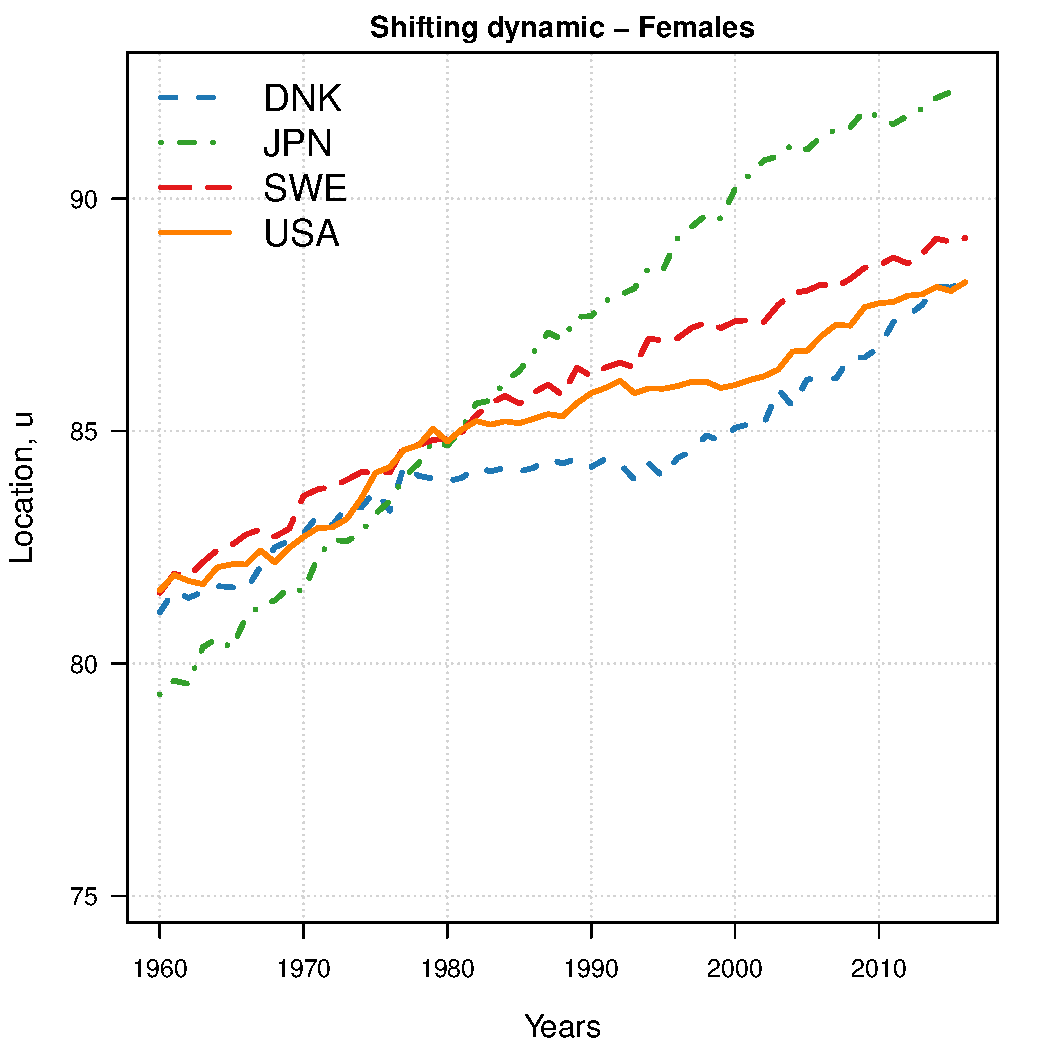
\includegraphics[scale=.4]{./Ch2/F3a.pdf}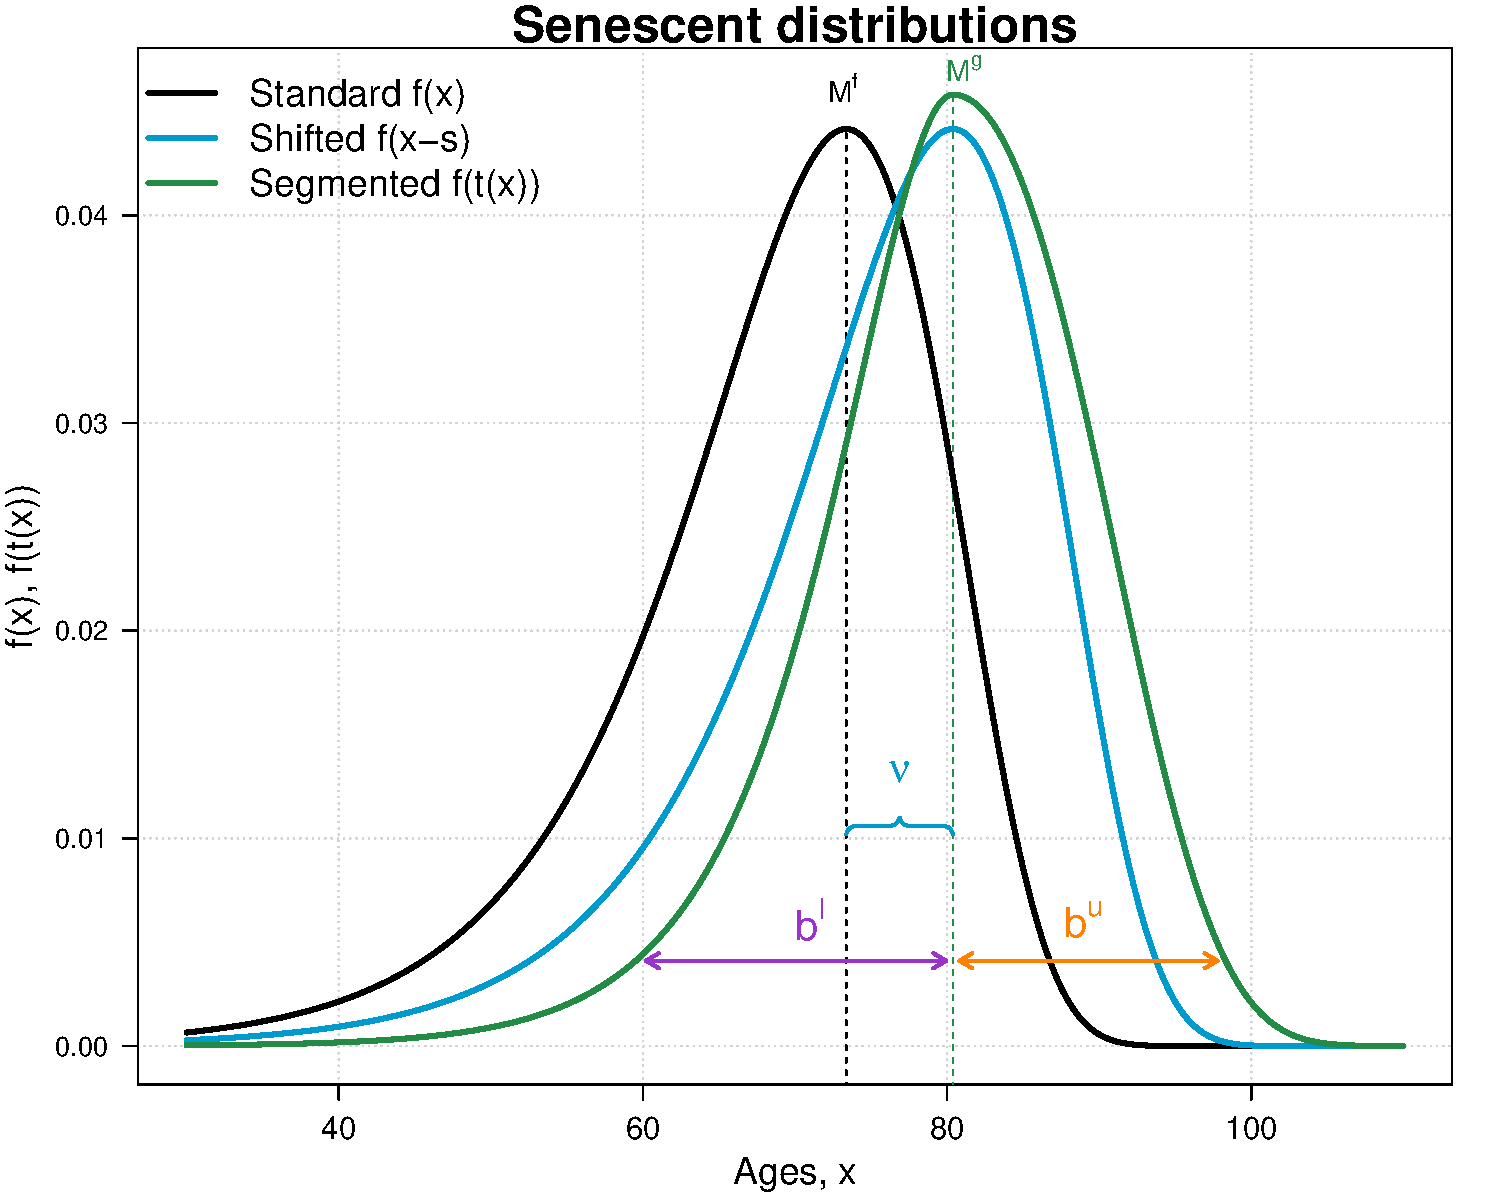
\includegraphics[scale=.4]{./Ch2/F3b.pdf}
	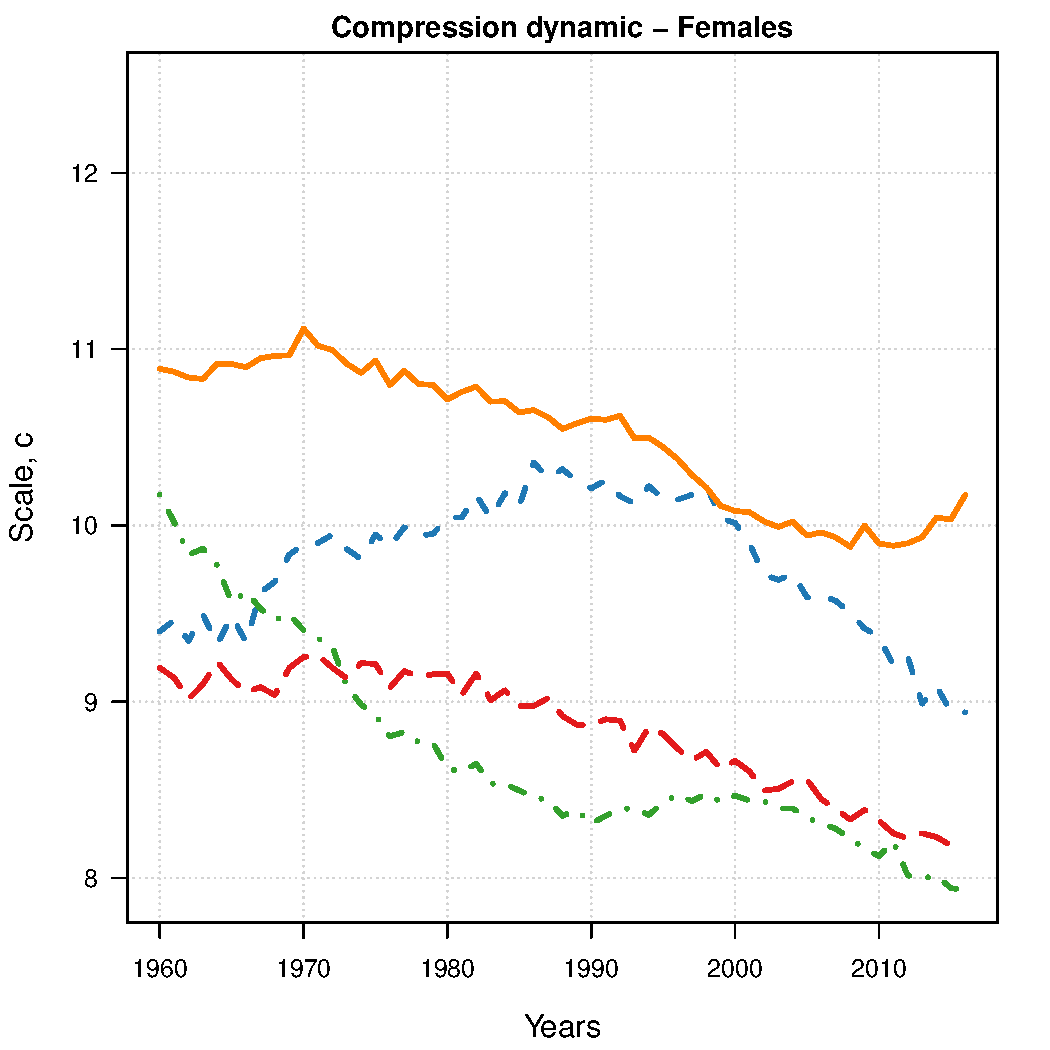
\includegraphics[scale=.4]{./Ch2/F3c.pdf}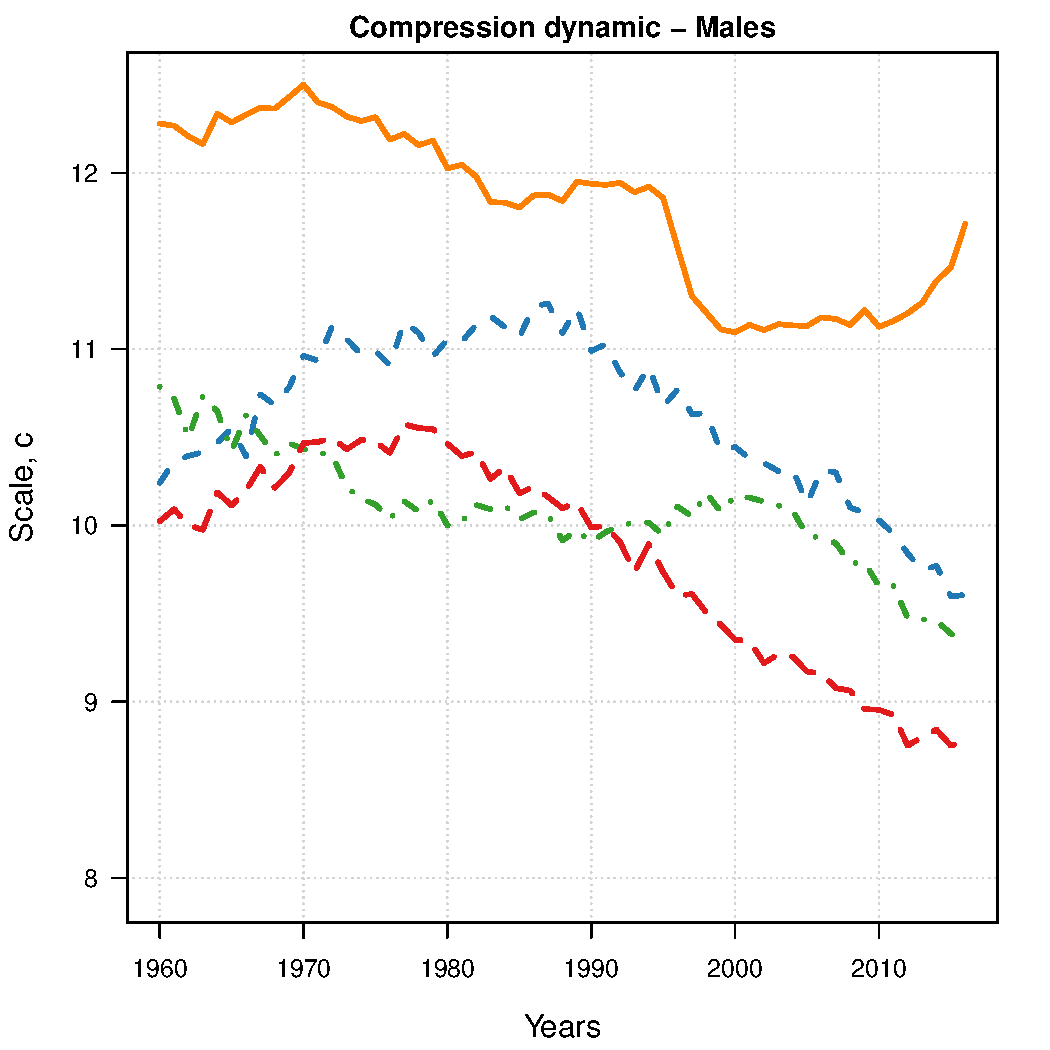
\includegraphics[scale=.4]{./Ch2/F3d.pdf}
	
	\caption{Estimated location $u$ and scale $c$ parameters of the Minimal Generalized Extreme-Value model for female (left) and male (right panels) adults aged 30-110+ in four high-longevity countries during 1960-2016.\\ \textit{Source (Figs.~\ref{Fig:Ch2LocScaParam}-\ref{Fig:Ch2LocSca6models}): Authors' calculations based on data from the \cite{HMD}}.}\label{Fig:Ch2LocScaParam}	
\end{figure}

From the top panels of Figure \ref{Fig:Ch2LocScaParam}, it is possible to determine the beginning of the shifting dynamic in the different countries by gender. For females, mortality started to shift before the 1960: indeed, the location parameter has been linearly increasing during all years in each country, albeit at different rates. Japanese females experienced the fastest rate of mortality postponement, which shows some signs of deceleration in most recent years; in addition, a lack of shifting mortality for Danish females clearly emerges during 1980-1995, a period coinciding with their stagnation of life expectancy \citep{christensen2010divergent,lindahl2016did,lindahl2016rise}. For males, the postponement of mortality started at different points in time in the four countries: while Japan was already experiencing this dynamic during the 1960s, the postponement started in the early 1970s in the USA, in the early 1980s in Sweden and in the early 1990s in Denmark.

From the bottom panels of Figure \ref{Fig:Ch2LocScaParam}, the compression dynamic of mortality can be assessed (decreasing values of $c$ correspond to compression). For females, a linear decreasing trend can be observed in Sweden and the USA, starting around the 1970s; in Japan, the decrease is very rapid until the 1990s, after which a period of stagnation occurred; and in Denmark, mortality first expanded for about twenty years at the beginning of the period (1965-1985), and then it started to compress again. For males, very different trends of compression, stagnation and expansion can be observed at different points in time. 

On top of assessing changes in the two dynamics, the LS parameters readily allow a cross-country comparison on the level of the two dynamics. A first interesting observation is that both females and males in the USA are lagging behind other countries in terms of both dynamics. The higher scale parameters in the USA correspond to a greater variability of the age-at-death distribution, which translates into a higher number of "premature" deaths (i.e.,~deaths occurring at young adult ages). Figure~\ref{Fig:Dx2016EV} in Appendix~\ref{Subsec:Ch2appD} reports the estimated MinGEV age-at-death distributions in 2016 for the four countries: the share of premature deaths for USA females and males is indeed higher than for the other three countries.

Another interesting observation is that location parameters for Denmark are below those for Sweden, while the scale parameters are higher. A possible interpretation is that the different smoking behaviour of Danish and Swedish has been a major reason for this difference. Denmark is one of the few high-income countries that experienced stagnation in life expectancy in recent decades \citep{lindahl2016rise}, which was paralleled by stagnation in lifespan inequality. Smoking has been indicated as the single most important factor in explaining the lower life expectancy  \citep{sun1994levetiden,lindahl2016did,jacobsen2004women,jacobsen2006causes} and the higher lifespan disparity in Denmark compared to Sweden \citep{aburto2018potential}.

Furthermore, Japanese women experienced the greatest shift of mortality as well as more compression compared to the other countries. The very fast improvements of mortality since the end of the Second World War have brought them to be the "best-practice" or most longevous population worldwide since the 1980s \cite[see][Fig.~2]{oeppen2002broken}. The Japanese age-profile of mortality has been shaped from over 35 years of best practice population, and is unique even among the closely competing countries such as South Korea and Hong Kong \citep{vallin2016highest,kontis2017future}.

Two important points are worth being mentioned here. First, the assessment of the shifting and compression dynamics would be the same if we had employed a different model of the LS family. Figure \ref{Fig:Ch2LocSca6models} in Appendix \ref{Subsec:Ch2appD} shows the location $u$ and scale $c$ rescaled estimates for six models of the LS family fitted on Swedish adult females and males. The Figure shows that the location and scale estimates are very consistent across models: the same patterns of shifting and compression dynamics emerge from the different LS models. Second, time trends of the location and scale parameters for the USA and Japan are in line with the empirical findings of shift and compression illustrated by \cite{canudas2008modal} and \cite{ouellette2011changes}: trends of the modal age at death and of the variability around (in the former) and above (in the latter) the mode closely resemble our results. Moreover, the trends of $u$ for Swedish and Danish females are remarkably similar to the trends of their temporary life expectancy between ages 50 and 85 \cite[see][Fig.~1(a)]{lindahl2016did}.

The analyses above, and in particular the assessment of the shifting dynamic, could not be performed based on the classic formulation of parametric models shown in the first column of Table \ref{Tab:Ch2LS}. Figure~\ref{Fig:LocScaVsStand} shows the Gamma-Gompertz (GG) estimates of the parameters $u$ (for the GG LS model) and $a$ (for the classic GG model) for males in the same four countries during 1960-2016. The estimates of $u$ for the GG LS model are very close to those of the MinGEV model shown in Figure~\ref{Fig:Ch2LocScaParam} (mean absolute percentage difference of 0.3\%). In the right panel of Figure \ref{Fig:LocScaVsStand}, the time trend of the parameter $a$ reflects changes in the level of the force of mortality at the starting age of the analysis. As such, it does not allow to disentangle mortality changes due to the shifting dynamic as captured by the $u$ parameter in the left panel. The trends of the two parameters (after reverting $u$ or $a$) are indeed not comparable: in the USA, for example, the trend of $a$ is quite erratic, while the parameter $u$ shows an unequivocal beginning of the shifting dynamic from the 1970s.  

\begin{figure}[!ht]
	\centering
	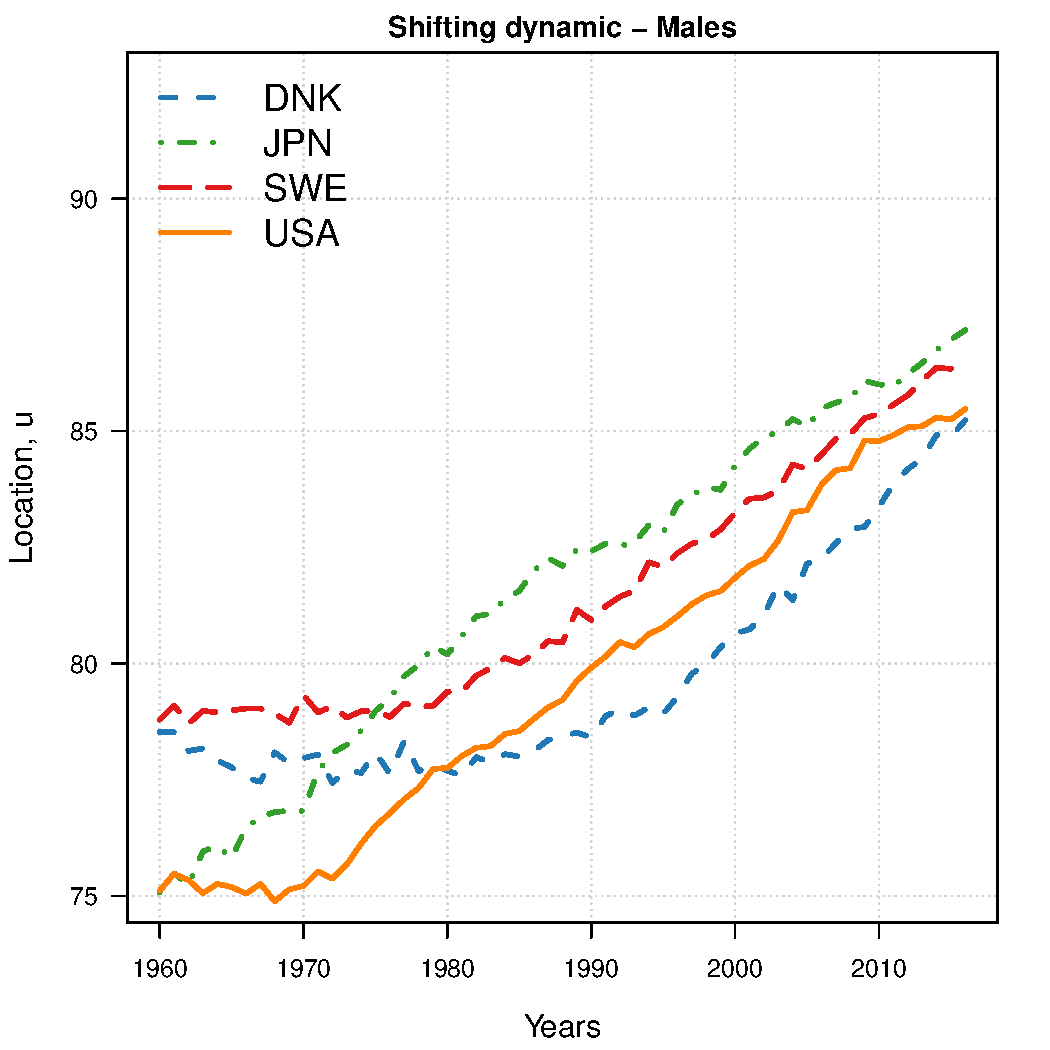
\includegraphics[scale=.4]{./Ch2/F4a.pdf}
	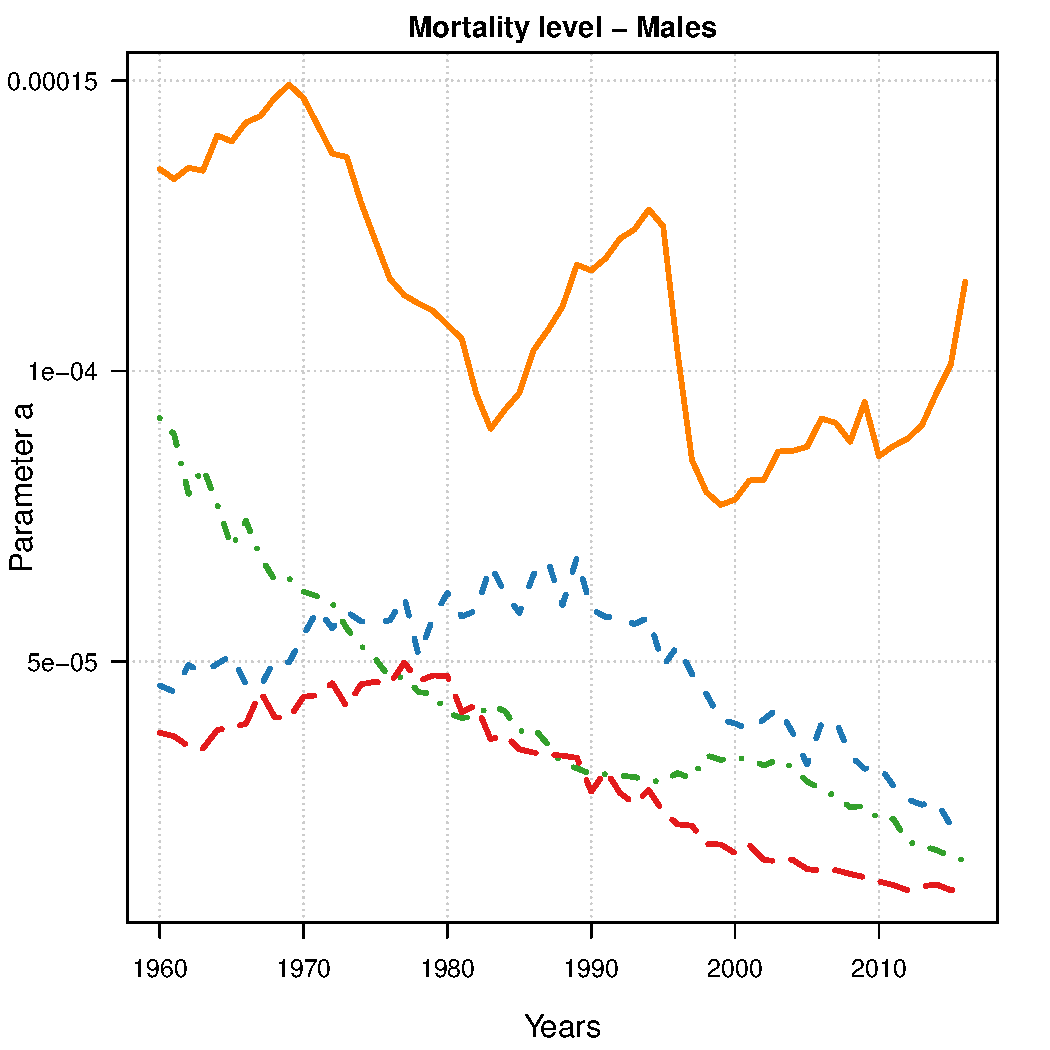
\includegraphics[scale=.4]{./Ch2/F4b.pdf}		
	\caption{Estimated Gamma-Gompertz parameters $u$ (LS model, left) and $a$ (classic model, right) for male adults aged 30-110+ in four high-longevity countries during 1960-2016. $\quad$ \textit{Note: the $y$-axis of the left panel is identical to the one in the upper-right panel of Fig.~\ref{Fig:Ch2LocScaParam} for comparison purposes.}}\label{Fig:LocScaVsStand}
\end{figure}

Finally, we present a decomposition of mortality changes into shift and compression effects for the four countries. Our methodology is based and extends the decomposition method introduced by \cite{bergeron2015decomposing} to the LS-like parameterization of the Gompertz model. Appendix~\ref{Subsec:Ch2appE} reports the formulas and computational procedures that we have used for this analysis. Figure~\ref{Fig:Decomposition} shows the decomposition of changes in life expectancy at age 30 by location (shifting) and scale (compression) contributions in the Gompertz model for females in the four countries from 1960 until 2015 in 5-year intervals.

\begin{figure}[!ht]
	\begin{center}
		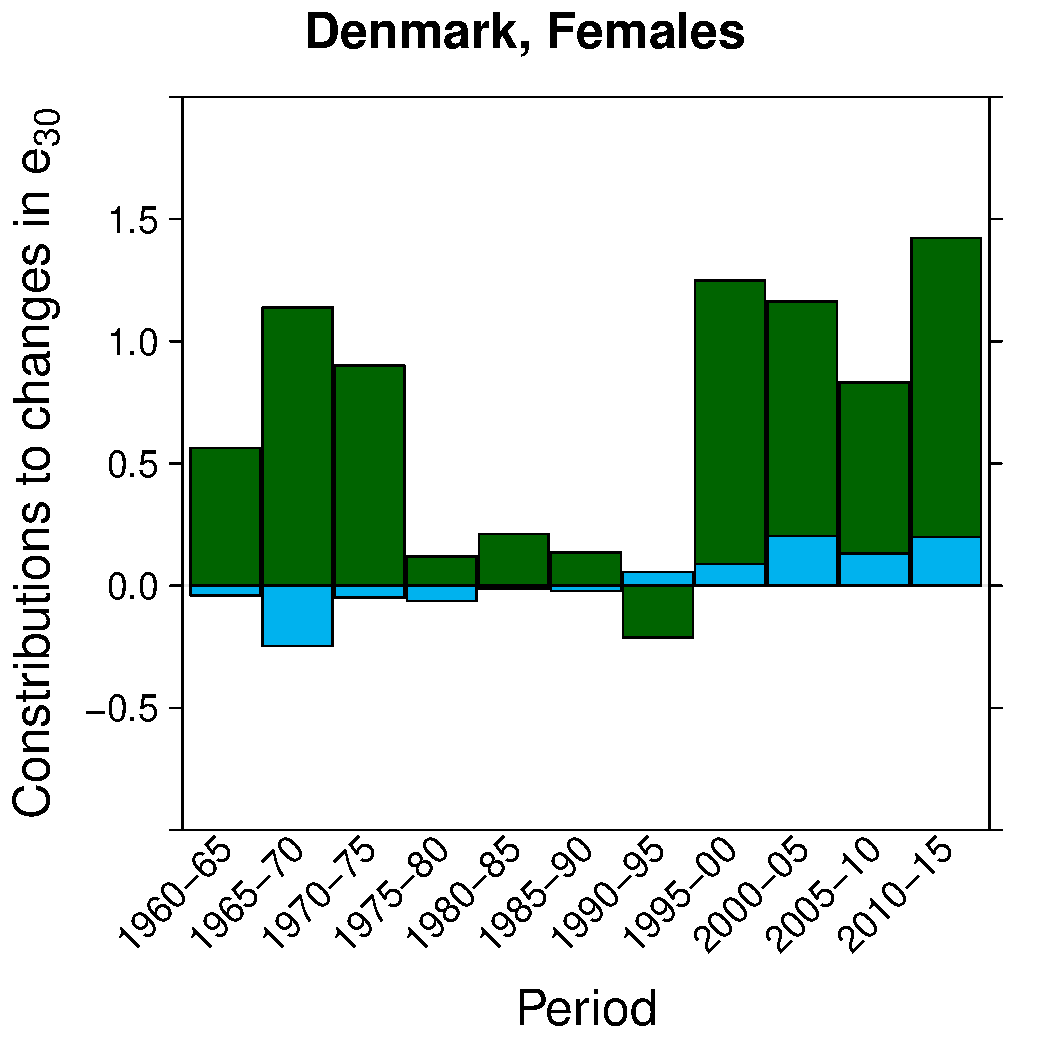
\includegraphics[scale=0.4]{./Ch2/F5b.pdf}
		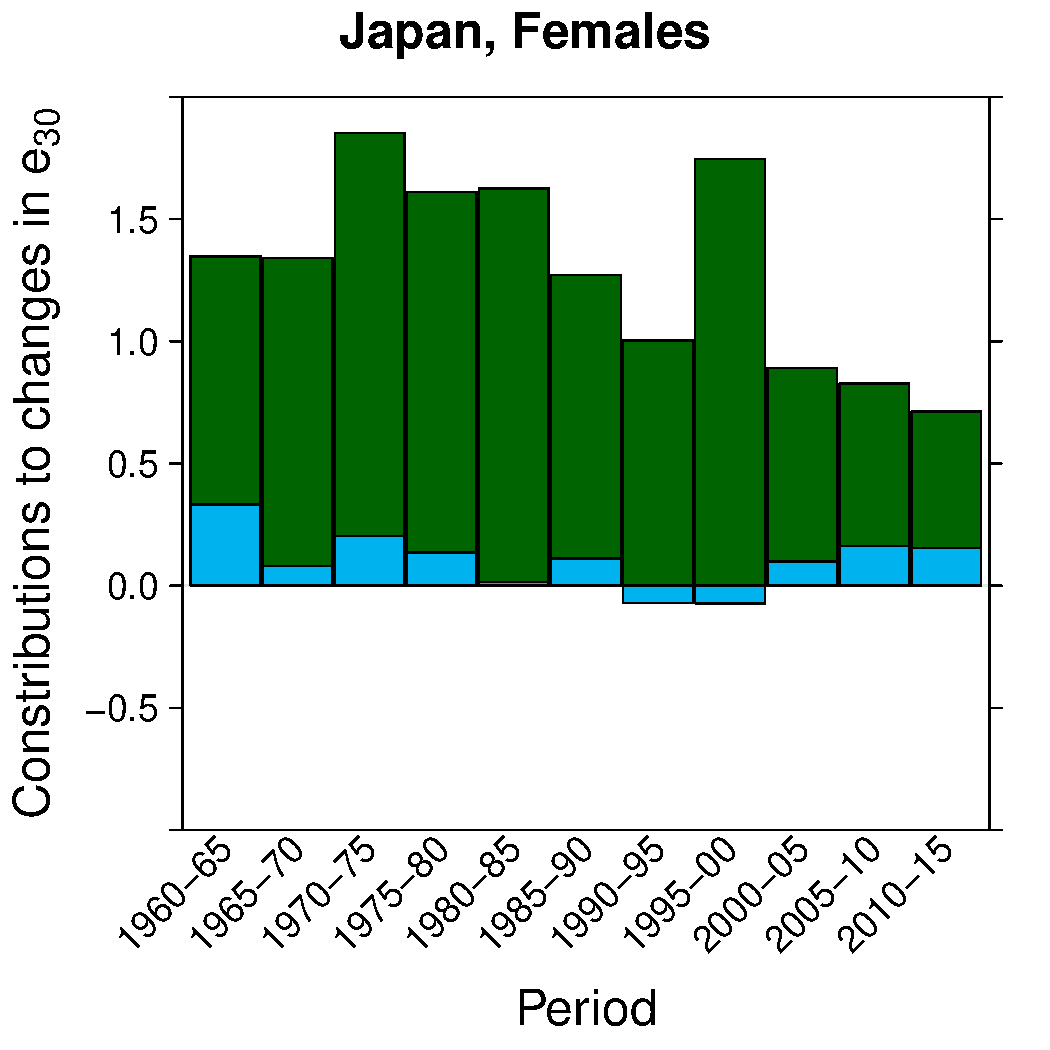
\includegraphics[scale=0.4]{./Ch2/F5d.pdf} 
		\vspace{0.4cm}
		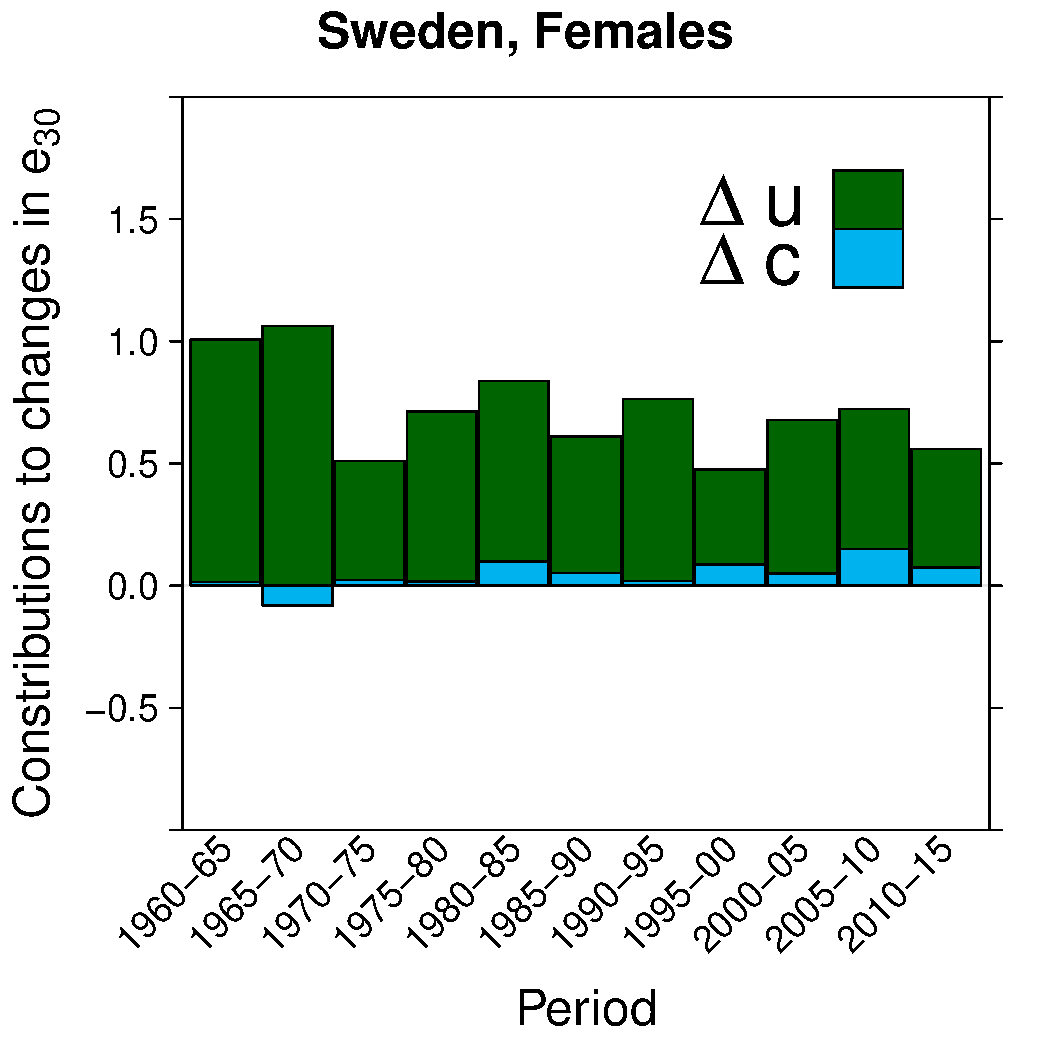
\includegraphics[scale=0.4]{./Ch2/F5a.pdf}
		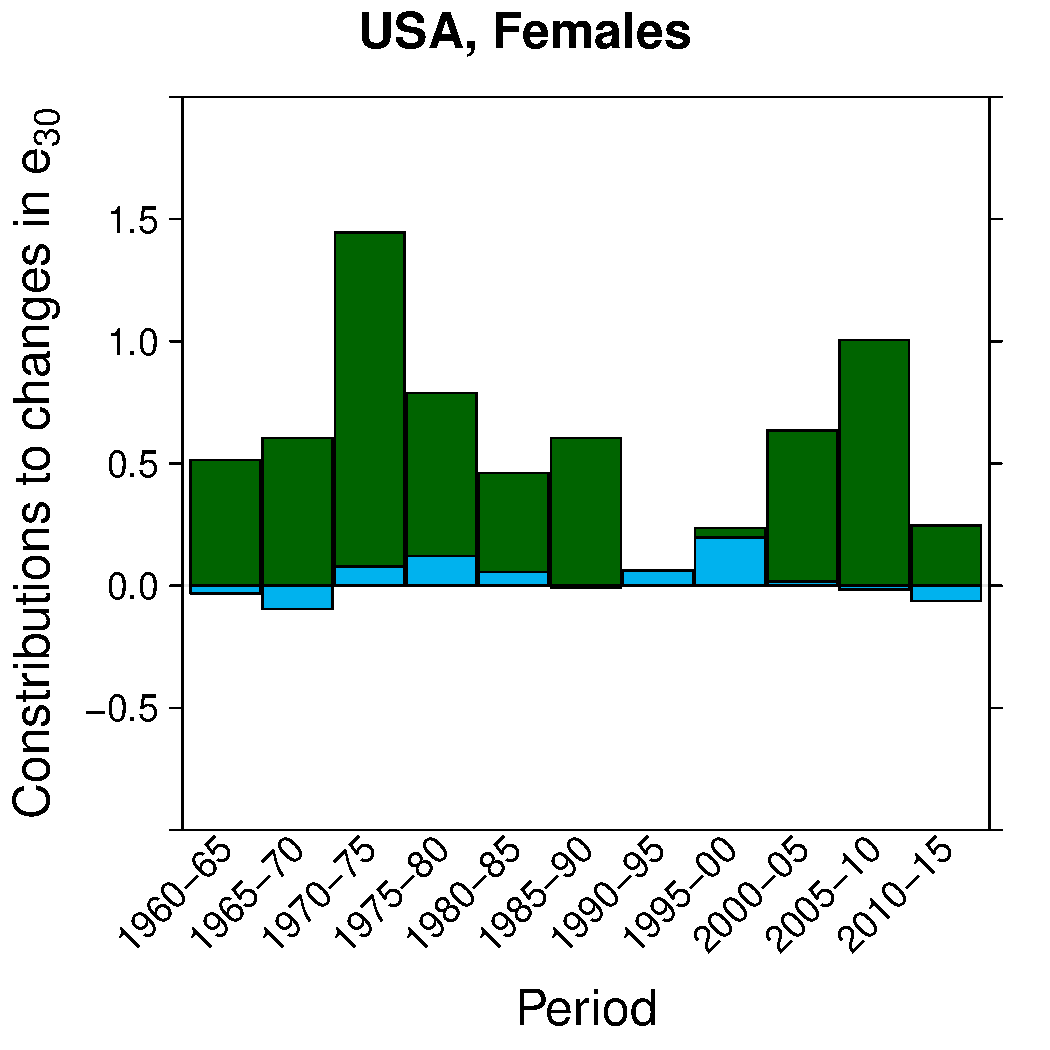
\includegraphics[scale=0.4]{./Ch2/F5c.pdf}
		
		\caption{Trends over time of the contributions of the location $u$ (green) and scale $c$ (light blue) Gompertz parameters to changes in female life expectancy at age 30 for females in Denmark, Japan, Sweden and the USA, 1960-2015.\label{Fig:Decomposition}} 	
	\end{center}  
\end{figure}

The Figure shows that changes in the location parameter, hence shifting mortality, are the main components driving changes in life expectancy during the period 1960-2015. Conversely, the contributions of changes in the scale parameter are limited, and even negatives in some periods. With respect to our previous discussions, the stagnation of the location parameter for Danish females between 1977 and 1995 is reflected in the small changes in life expectancy during this period. Moreover, the fast increase of the location parameter experienced by Japanese females has been the main contributor to the remarkable gains in life expectancy. These results are in line with those reported by \citeauthor{bergeron2015decomposing} (\citeyear{bergeron2015decomposing}, Fig.~7, Appendix C).

\subsection{Correlation and bias of parameter estimates}
\label{Subsec:Ch2subsec3.2}

It is well known that a high correlation between the estimators of model parameters is an undesirable property, as "\textit{it shows a kind of inaccuracy of the estimators}" \cite[][p.~588]{gupta1994location}. Reducing the correlation of the maximum likelihood estimators (MLE) of parametric models is therefore a beneficial task, as it improves parameter interpretability and reduces estimation bias. In particular, \cite{gupta1994location} have shown that  location--scale distributions can generally be re-parameterized so that the maximum likelihood estimators are asymptotically independent.

\cite{missov2015gompertz} have shown that the MLE of the parameters $a$ and $b$ of the classic Gompertz model in Equation~(\ref{GompertzMu}) are highly (negatively) correlated. This is in general true for the parametric models in Table~\ref{Tab:Ch2LS} that are expressed in their classic notation $\mu(x)$. Figure~\ref{Fig:Ch2CorrNOR} shows the MLE of the typical $a$ and $b$ parameters of the Gamma-Gompertz, Gompertz and Kannisto mortality models for the thirty-three Human Mortality Database (HMD) countries listed above from 1960 until the most recent year by gender. Each point on the graph corresponds to a set of estimated parameters for a single country in a given year. 

\begin{figure}[!ht]
	\centering
	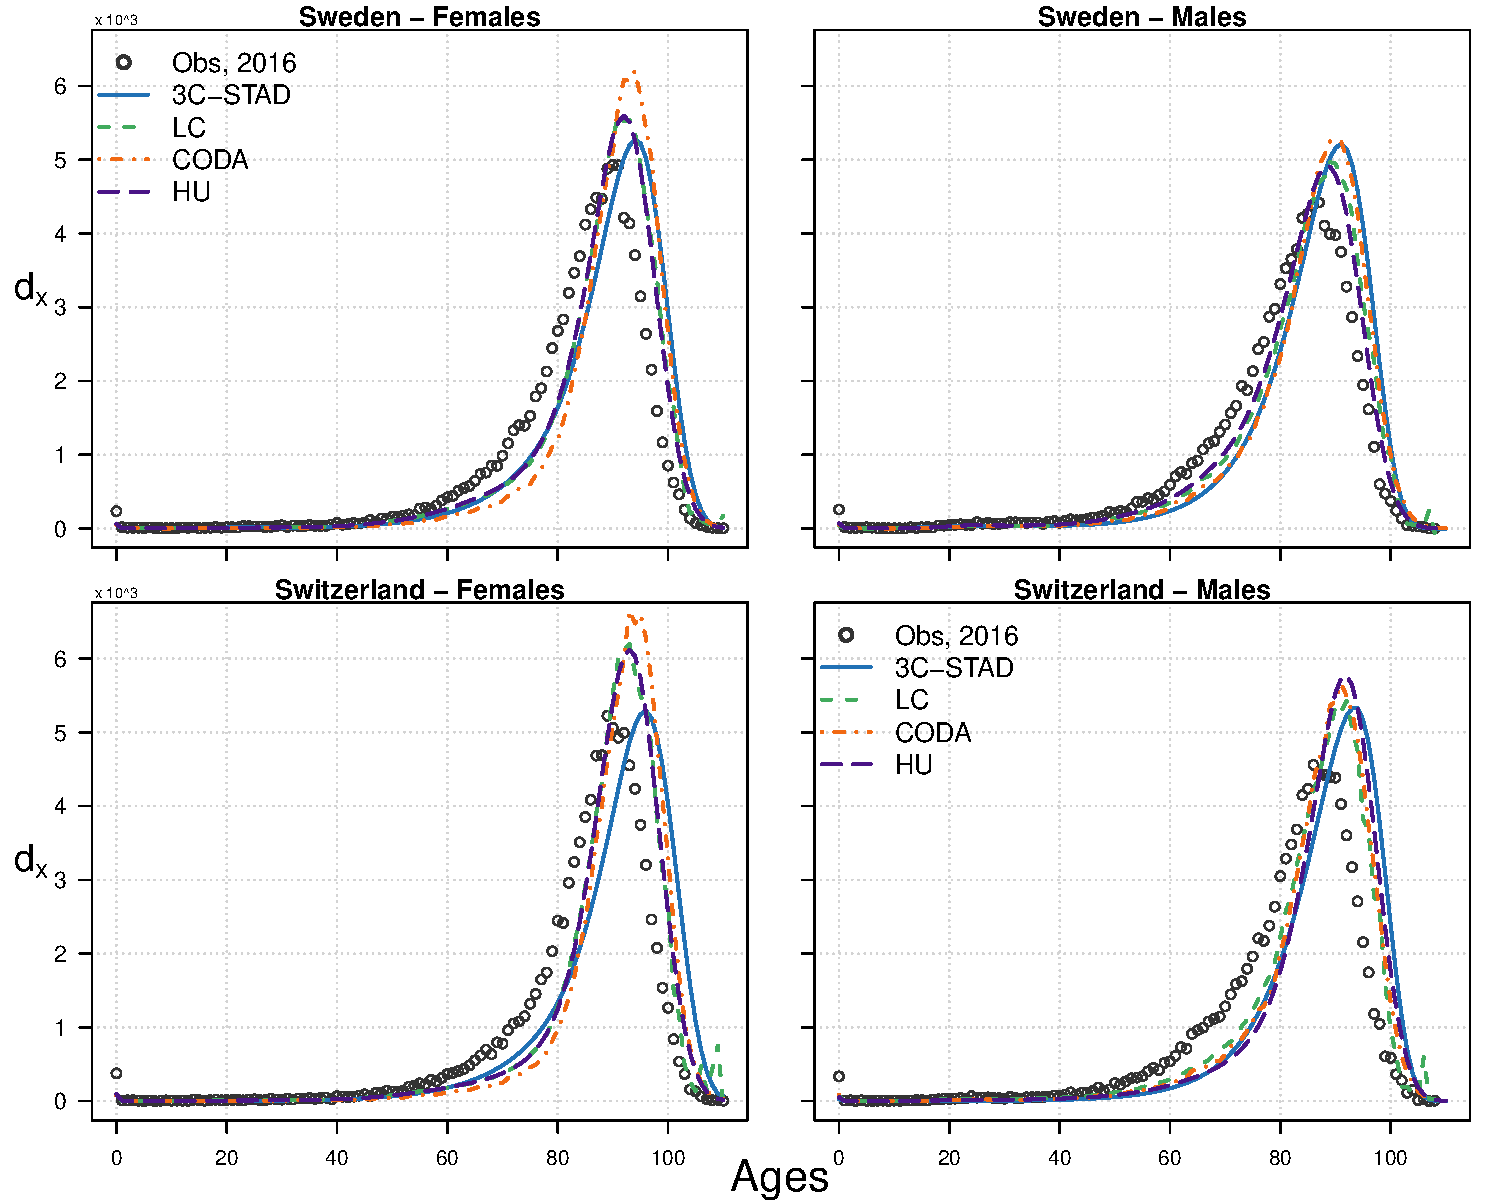
\includegraphics[scale=.7]{./Ch2/F6.pdf}
	\caption{Maximum likelihood estimates and $R^2$ of a linear model for the classic parameters $a$ and $b$ for the Gamma-Gompertz, Gompertz and Kannisto model for thirty-three HMD countries from 1960 until the most recent year by gender. The $a$ parameter was transformed in $a^{0.1}$ to linearise the relationship for the two Gompertz cases.}\label{Fig:Ch2CorrNOR}
	
\end{figure}

The estimated parameter $b$ tends to decrease as $a$ increases for all models, following a power function for the two Gompertz's specifications and a linear function for the Kannisto model. The variability around the two estimated parameters is very small: indeed, the $R^2$ of a linear model between $a$ and $b$ (after a suitable power transformation of the parameter $a$ for the two Gompertz cases) is always very high (average $R^2$ of 0.90). 

This rather high correlation between the estimators of classic parametric models can be reduced by re-parameterizing them in terms of the LS family. Figure~\ref{Fig:Ch2CorrLS} shows the MLE of the LS parameters $u$ and $c$ for the same models, countries and years by gender. From the graphs, it is clear that the relationship between the LS estimates is much weaker than for the classic ones. The variability around the LS parameters is higher, and the $R^2$ of the linear regression between $u$ and $c$ is significantly reduced (average $R^2$ of 0.31). Furthermore, the relationship is not always negative as in the previous case: for the Kannisto model, increases in $u$ tend to correspond to increases in $c$. 

\begin{figure}[!ht]
	\centering
	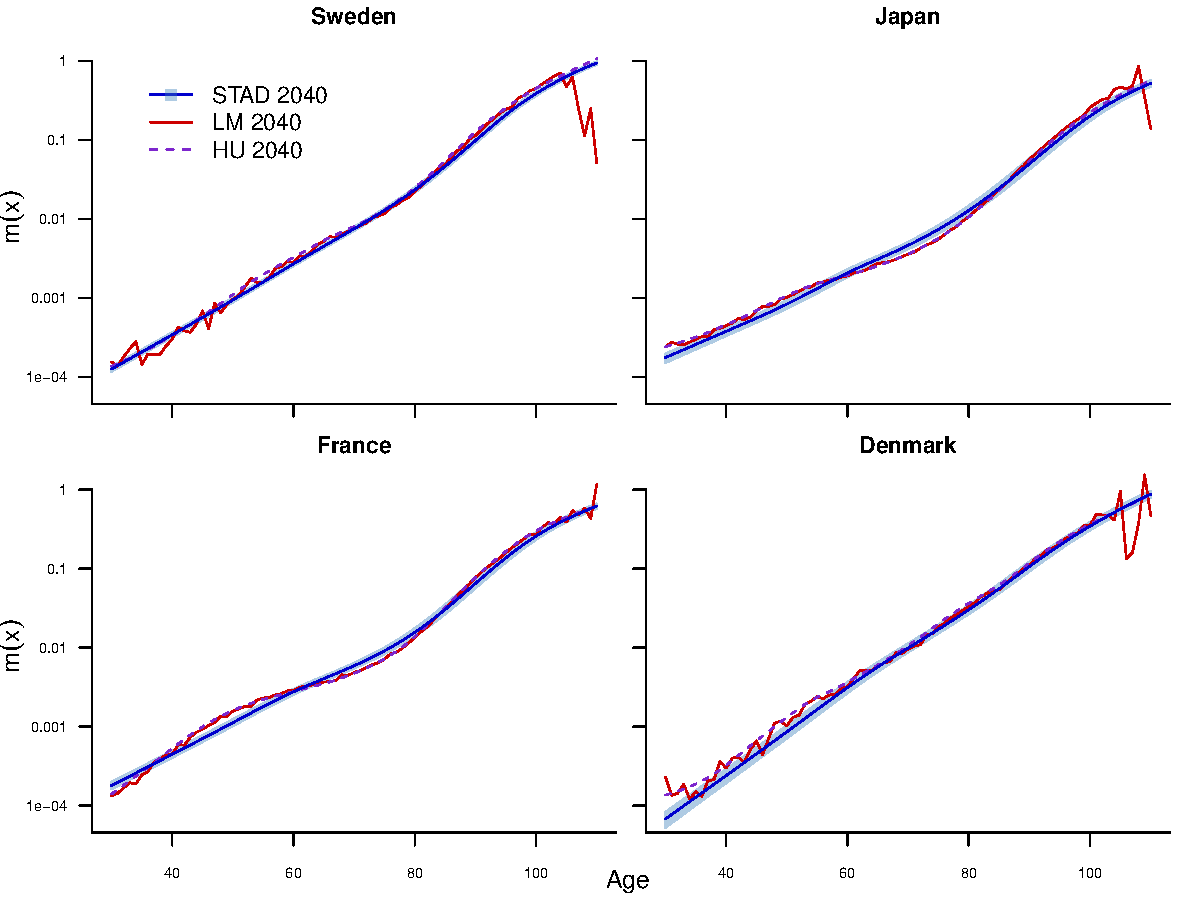
\includegraphics[scale=.7]{./Ch2/F7.pdf}
	\caption{Maximum likelihood estimates and $R^2$ of a linear model for the LS parameters $u$ and $c$ for the Gamma-Gompertz, Gompertz and Kannisto model for thirty-three HMD countries from 1960 until the most recent year by gender.}\label{Fig:Ch2CorrLS}
	
\end{figure}

The weaker relationship of the LS estimates \textit{between} countries is generated by a lower correlation of $u$ and $c$ with respect to $a$ and $b$ \textit{within} countries. Figure \ref{Fig:Ch2CorrWithinCou} shows the within-country absolute correlation of the two set of estimated parameters for the three-models: each point on the graph corresponds to the absolute correlation of the classic and LS parameters within one country during all the years considered in the analysis (1960 until the most recent available year) by gender.  The great majority of points in Figure \ref{Fig:Ch2CorrWithinCou} fall below the diagonal, confirming that the absolute correlation between estimators of classic models' parameter can be significantly reduced by using the LS family.

\begin{figure}[!ht]
	\centering
	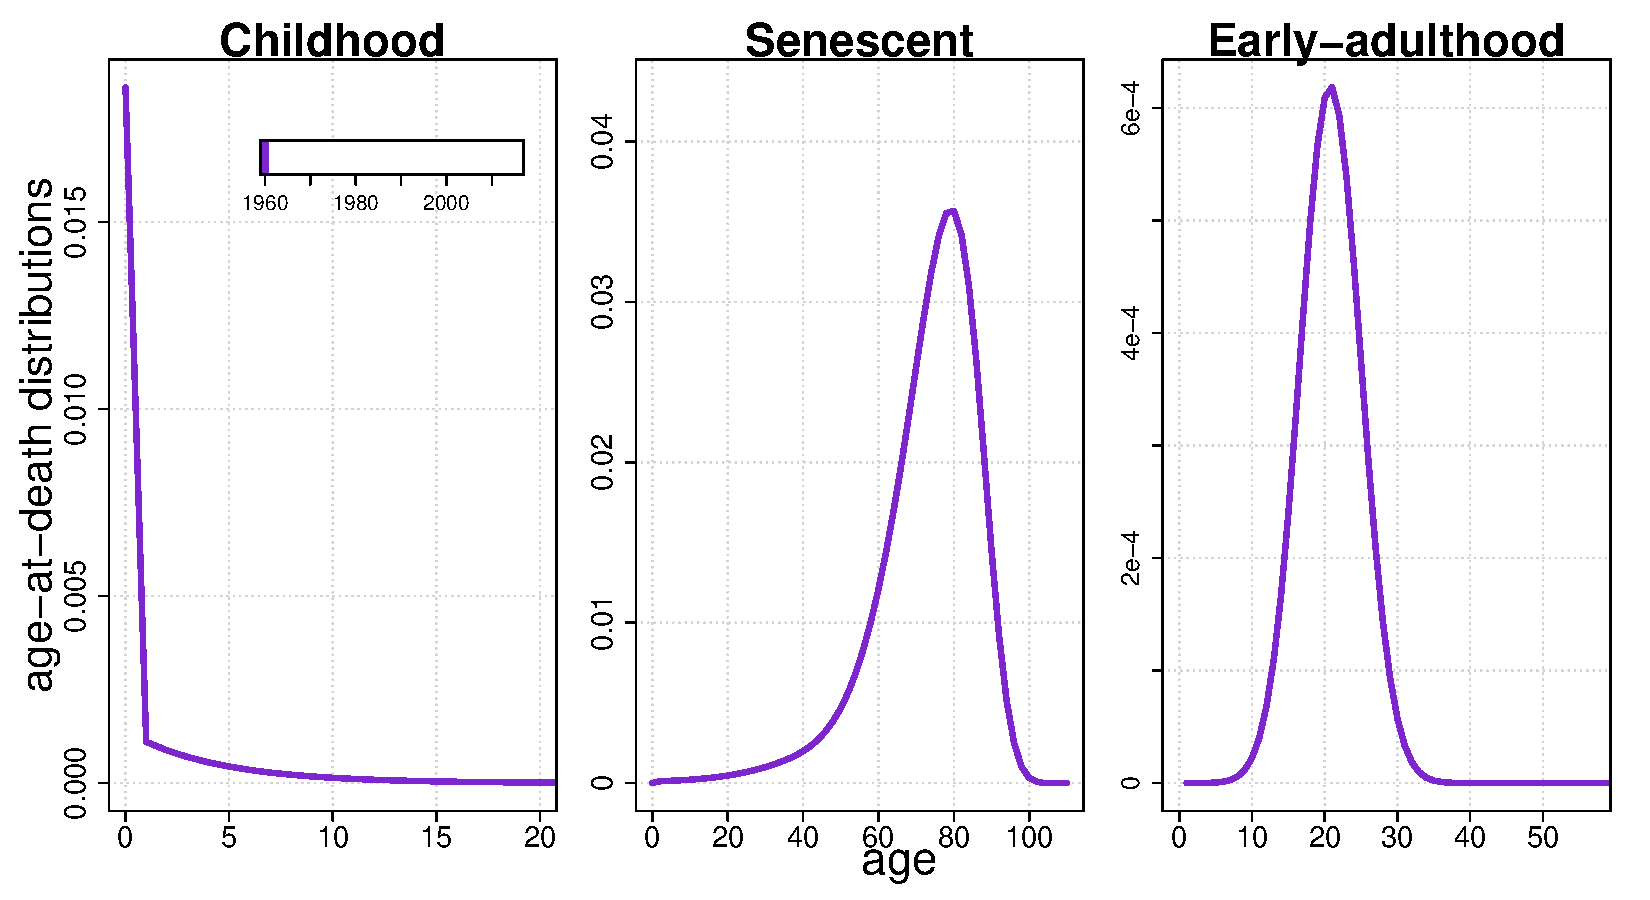
\includegraphics[scale=.7]{./Ch2/F8.pdf}
	\caption{Within-country absolute correlation of the classic and LS parameterization of the Gamma-Gompertz, Gompertz and Kannisto model for thirty-three HMD countries from 1960 until the most recent year by gender.}\label{Fig:Ch2CorrWithinCou}
	
\end{figure}

Finally, we perform an experiment that demonstrates the reduction of estimation bias when using the LS family versus the classic models' parameterization. Specifically, we consider Swedish adult female mortality in 2000, and we estimate the Weibull, Logistic and Gompertz LS parameters $u$ and $c$. We consider these estimates to be the "true" model parameters, and we derive the corresponding true $a$ and $b$ of the classic models via the formulas in Table~\ref{Tab:Ch2LS}. Then, we produce 100 simulations of age-specific Poisson death counts using the true hazard and the observed exposure times. For each simulation, we estimate the LS and classic model's parameters, and we compute the relative absolute bias (AB) for each parameter $\theta$ using the formula: 
\begin{equation}\label{Eq:AB}
\mathrm{AB} = \frac{|\,\hat{\theta}-\theta\,|}{\theta} \, ,
\end{equation}
where $\hat{\theta}$ is the estimated value of the true parameter $\theta$ \citep{pletcher1999model}. Table \ref{Tab:Ch2Simul} reports the AB averaged over 100 simulations for the classic and LS parameters' estimates of the Weibull, Logistic and Gompertz models.

\begin{table}[!ht]
	\centering
	\caption{Relative absolute bias (AB, in percentage terms) averaged over 100 simulations for the Weibull, Logistic and Gompertz classic parameters $a$ and $b$, and the LS parameters $u$ and $c$ estimated on simulated Swedish adult female deaths in 2000.}
	\label{Tab:Ch2Simul}
	\begin{tabular}{@{}lcccc@{}}
		\toprule
		& \multicolumn{4}{c}{AB}             \\ \cmidrule(l){2-5} 
		\multicolumn{1}{l|}{Model $\quad\quad$}    & a & \multicolumn{1}{c|}{b} & u & c \\ \midrule
		\multicolumn{1}{l|}{Weibull}  & 0.043  &  \multicolumn{1}{c|}{0.294}  &  0.001 &  0.005 \\ \rowcolor{my-grey}	
		\multicolumn{1}{l|}{Logistic} & 0.344  & \multicolumn{1}{c|}{0.352}  &  0.044 &  0.351 \\
		\multicolumn{1}{l|}{Gompertz} & 3.048  & \multicolumn{1}{c|}{0.327}  &  0.037 &  0.326 \\ \bottomrule
	\end{tabular}
\end{table}

The Table shows that the AB for the LS estimates is always lower than for the classic model parameterization: employing the LS formulas improves the precision of parameters' estimates. These results are in line with those of \citeauthor{missov2015gompertz}, who performed a somewhat similar simulation experiment for the Gompertz model and showed that "\textit{a model misspecification leads to a relatively small bias in estimated $M$} [i.e.,~$u$ in the LS framework] \textit{in comparison to the bias in the estimated $a$}" \cite[][p.~1039]{missov2015gompertz}.


\section{Discussion and conclusion}
\label{Sec:Ch2sec4}

In this article, we have shown that many mortality models used in the demographic and actuarial literature can be re-parameterized in terms of a general and flexible family of models, the family of location--scale (LS) models. The models belonging to this family are characterized by two parameters that have a direct demographic interpretation: the location and scale parameters capture the shifting and compression dynamics of mortality changes. 

The study of compression and shifting mortality is an important issue in demographic research, as both dynamics translate differently into survival function, mortality density and hazard distributions \citep{bergeron2015decomposing}. Mortality compression is associated with a rectangularization of the survival curve and with decreasing variability in the distribution of ages at death \citep{wilmoth1999rectangularization,cheung2005three}. Mortality shifting is associated with a parallel shift of the force of mortality to lower ages \citep{bongaarts2005long} and of the death distribution to higher ages \citep{canudas2008modal}, while retaining their original shape. As we have shown in Section \ref{Subsec:Ch2subsec3.1}, the estimation of the parameters of the LS family allows an assessment of the level and trend of these two mortality dynamics.

As such, re-parameterizing classic models in their LS formulation is very useful in aiding parameter interpretability and comparability across different populations. We have shown as illustration in Section \ref{Subsec:Ch2subsec3.1} the analysis of the shifting and compression dynamics of mortality changes in four high-longevity countries by gender during 1960-2016: the LS estimated parameters readily allow to examine and compare the two dynamics within and between countries.

In addition, the LS parameterization has an important statistical advantage over classic models: the rather high correlation between estimators of classic models' parameterization is significantly reduced within the LS framework, and thus statistical estimation is facilitated. The lower correlation, in turn, further improves parameter interpretability and reduces estimation bias. As an illustration, we have shown in Section \ref{Subsec:Ch2subsec3.2} that the correlation of the classic Gamma-Gompertz, Gompertz and Kannisto parameters for females and males aged 30-110+ in thirty-three Human Mortality Database countries is significantly higher than the LS parameterization, both within and between countries. Moreover, we performed simulation experiments to demonstrate the reduction of estimation bias for the Weibull, Logistic and Gompertz models when using the LS framework instead of the classic models' formulas.

Another potentially important advantage deriving from the lower correlation is that the LS parameters could be forecasted more appropriately. The main advantages of using parameterization functions for forecasting mortality are the smoothness of forecast rates across age and the interpretability of the model's parameters \citep{bell1997comparing,booth2008mortality}. Nevertheless, forecasting via well-known laws of mortality has been very limited due to the very high correlation between parameter's estimators \citep{booth2008mortality}. The lower correlation of the LS estimators could thus overcome this relevant issue. Parametric forecasts of mortality obtained with classic and the LS models are beyond the scope of the current paper and will be explored and compared in future work.

Although we have shown that several mortality models belong to the LS family, it should be noted that the family does not embrace the full spectrum of parametric  models. Additive hazard models developed for adult mortality (e.g. the Makeham and the Gamma-Gompertz-Makeham models) as well as for the entire age range, such as the \cite{siler1979competing}, the \cite{heligman1980age} and the CoDe \citep{de2016new} models,  do not belong to the LS family.

Nevertheless, the LS family reconciles several parametric mortality models under a unique framework, it readily allows the assessment of the shifting and compression dynamics of mortality changes, and it aids statistical estimation due to lower correlation between estimates of the model parameters. In turn, the latter could be further exploited for forecasting purposes. Re-parameterizing classic demographic models in terms of the LS family therefore offers great advantages, and the family should be considered for parametric mortality analysis.

% ---- Appendix ----
% --------------------------------------------

\section{Appendix}\label{Sec:Ch2Appendix}

\subsection{Weibull and the log--location--scale family}
\label{Subsec:Ch2appA}

Here, we provide a similar derivation of Section \ref{Subsec:Ch2subsec2.3} to show that the Weibull model belongs to the log--location--scale (LLS) family of mortality models.

Among its various parameterization, the Weibull model can be expressed in the form:
\begin{eqnarray}\label{WeibullMu}
\mu (x)=ab \, (ax)^{b-1} \, , \quad x>0  \, ,
\end{eqnarray}
where $a>0$ and $b>0$ are parameters \citep{lawless2011statistical}. From the life-table functions introduced in Section \ref{Subsec:Ch2subsec2.1}, we can then derive the density function $f(x)$ of the Weibull model:
\begin{eqnarray} \label{WeibullDens}
f(x) = \mu (x)l(x)  = \frac{b}{x}  \, (ax)^{b}  \, \mathrm{exp} \left [ - (ax)^{b} \right ] .
\end{eqnarray}

The Weibull model can be re-parameterized in terms of the LLS family. In particular, the LLS Weibull model for the force of mortality is:
\begin{eqnarray}\label{WeibullLS}
\mu(x) = \frac{1}{c\,x} \, \mu_{LLS} \left(\frac{\ln(x)-u}{c} \right) = \frac{1}{c\,x} \, \mathrm{exp} \left (\frac{\ln(x)-u}{c} \right ) \, ,
\end{eqnarray}
where $u \in \mathbb{R}$ and $c > 0$ are the location and scale parameters, respectively. The corresponding LLS density function of the Weibull model can be expressed as:
\begin{eqnarray}\label{WeibullDensLS}
f(x) &=& \frac{1}{c\,x} \, f_{LLS} \left ( \frac{\ln(x)-u}{c} \right ) \notag \\ &=& \frac{1}{c\,x} \, \mathrm{exp} \left [ \frac{\ln(x)-u}{c} - \mathrm{exp} \left ( \frac{\ln(x)-u}{c} \right ) \right ] 
\, .
\end{eqnarray}

Indeed, if we let the location and scale parameters be $u =   - \mathrm{ln} (a)$ and $c=\frac{1}{b}$, and we substitute them in Equations (\ref{WeibullLS}) and (\ref{WeibullDensLS}), we obtain the classic Weibull formulas in Equation (\ref{WeibullMu}) and (\ref{WeibullDens}). As such, the Weibull model belongs to the LLS family of mortality models defined in Equations (\ref{Eq:Ch2LSLpdf}) and (\ref{LSLMmux}). 


\subsection{Location--scale functional form of twelve parametric models of mortality }\label{Subsec:Ch2appB}

Table \ref{Tab:Ch2LSfx} presents the classic, location--scale (LS) and log--location--scale (LLS) functional forms $f(x)$, $f_{LS}(\cdot)$ and $f_{LLS}(\cdot)$ of the mortality models presented in Section \ref{Subsec:Ch2subsec2.4}. 

\begin{table}[!ht]
	\begin{center}
		\caption{Mortality models belonging to the location--scale (LS) and log--location--scale (LLS) families, and models closely related to them, together with their parameterization in terms of the classic, LS and LLS functional forms $f(x)$, $f_{LS}(x)$ and $f_{LLS}(x)$.}\label{Tab:Ch2LSfx}
		
		\scriptsize
		\begin{tabular}{l c c}						
			
			\toprule
			
			\begin{tabular}[l]{@{}l@{}}\textbf{Models belonging}\\ \textbf{to the LS family}\end{tabular} & $\qquad$ $\boldsymbol{f(x)}$ $\qquad$ &    $ \boldsymbol{\frac{1}{c}\, f_{LS} \left (\frac{x-u}{c} \right ) }$        \\	
			\midrule	 \\
			
			Logistic  & $\frac{b \, \mathrm{exp}(a+bx)}{\left[1+ \mathrm{exp}(a+bx)\right]^2 }$   & $ \frac{1}{c}\, \frac{\mathrm{exp}(\frac{x-u}{c})}{\left[1+\mathrm{exp}(\frac{x-u}{c})\right]^2} $    \\ \\ \rowcolor{my-grey}
			
			Normal  & $ \frac{1}{\sigma} \phi (\frac{x-\lambda}{\sigma})$ & $\frac{1}{c}\,\phi (\frac{x-u}{c})      $  \\ \\		
			
			\begin{tabular}[c]{@{}l@{}}Smallest\\ Extreme-Value \end{tabular} & $\frac{1}{\sigma} \, \mathrm{exp} \left[\frac{x-\lambda}{\sigma} - \mathrm{exp} \left(\frac{x-\lambda}{\sigma} \right) \right] $  & $\frac{1}{c}\,\mathrm{exp} \left[\frac{x-u}{c} - \mathrm{exp} \left(\frac{x-u}{c} \right) \right]$    \\ \\  \rowcolor{my-grey}
			
			\begin{tabular}[c]{@{}l@{}}Largest\\ Extreme-Value \end{tabular} & $\frac{1}{\sigma} \, \mathrm{exp} \left[- \frac{x-\lambda}{\sigma} - \mathrm{exp} \left(-\frac{x-\lambda}{\sigma} \right) \right]$  & $\frac{1}{c}\,\mathrm{exp} \left[- \frac{x-u}{c} - \mathrm{exp} \left(-\frac{x-u}{c} \right) \right]$   \\ 
			
			\bottomrule					
			
			\\
			
			\toprule
			
			\begin{tabular}[c]{@{}l@{}}\textbf{Models belonging}\\\textbf{to the LLS family}\end{tabular} & $\qquad$ $\boldsymbol{f(x)}$ $\qquad$ &    $\boldsymbol{\frac{1}{c\,x} \, f_{LLS} \left (\frac{\ln(x)-u}{c} \right )}$   \\	
			\midrule	\\
			
			
			Weibull $\qquad$  & $ab \, (ax)^{b-1} \, \mathrm{exp} \left [ - (ax)^b \right ] $   & $ \frac{1}{c\,x}\, \mathrm{exp} \left[ \frac{\ln(x)-u}{c} - \mathrm{exp} \left( \frac{\ln(x)-u}{c} \right) \right] $   \\  \\ \rowcolor{my-grey}
			
			Log-Logistic  & $ \frac{b}{x} \, \frac{\mathrm{exp}(a+b\ln(x))}{\left [ 1+\mathrm{exp}(a+b\ln(x))\right ]^2} $   & $\frac{1}{c\,x}\,\frac{\mathrm{exp}(\frac{\ln(x)-u}{c})}{\left[1+\mathrm{exp}(\frac{\ln(x)-u}{c})\right]^2}$    \\ \\
			
			Log-Normal  & $ \frac{1}{\sigma\,x}\, \phi (\frac{\ln(x)-\lambda}{\sigma}) $ & $\frac{1}{c\,x}\,\phi (\frac{\ln(x)-u}{c}) $        \\ 						
			
			\bottomrule					
			
			\\
			
			\toprule
			
			\begin{tabular}[c]{@{}l@{}}\textbf{Models related}\\ \textbf{to the LS family}\end{tabular} & $\qquad$ $\boldsymbol{f(x)}$ $\qquad$ &  \textbf{LS-like}  $\boldsymbol{f(x)}$       \\	
			\midrule	 \\
			
			Gompertz $\qquad$  & $a \, \mathrm{exp} \left [ bx -\frac{a}{b} (e^{bx}-1) \right ]$  & $\frac{1}{c}\,\mathrm{exp} \left [ \frac{x-u}{c} - \mathrm{exp} \left ( \frac{x-u}{c} \right ) + \mathrm{exp} \left ( - \frac{u}{c} \right ) \right ] $  \\ \\ \rowcolor{my-grey}
			
			Gamma-Gomp & $ \frac{a\, \mathrm{exp}(bx)}{\left\{ 1+\frac{a}{b}\gamma \left[\mathrm{exp}(bx) -1 \right] \right\}^{\frac{1}{\gamma}+1}}$ $\qquad$ & $\frac{1}{c}\, \frac{ \mathrm{exp} \left ( \frac{x-u}{c} \right ) }{ \left\{ 1+ \gamma \left[ \mathrm{exp} \left( \frac{x-u}{c} \right) - \mathrm{exp} \left( -\frac{u}{c} \right) \right]  \right\}^{\frac{1}{\gamma}+1} }$   \\ \\
			
			
			Kannisto  & $\frac{\mathrm{exp}(a+bx)}{\left[1+ \mathrm{exp}(a+bx)\right]^{\frac{1}{b}+1} }$   & $ \frac{\mathrm{exp}(\frac{x-u}{c})}{\left[1+\mathrm{exp}(\frac{x-u}{c})\right]^{1+c}} $    \\ \\  \rowcolor{my-grey}
			
			\begin{tabular}[c]{@{}l@{}} Minimal Generalized\\ Extreme-Value\end{tabular}
			& $   \frac{1}{\sigma}\,\frac{\mathrm{exp}\left\{ -\left[  1+\xi \left ( - \frac{x-\lambda}{\sigma} \right ) \right]^{-\frac{1}{\xi}} \right\}}{\left [ 1+ \xi  \left (- \frac{x-\lambda}{\sigma} \right )  \right ]^{\frac{1}{\xi}+1}}  $ & $  \frac{1}{c}\, \frac{\mathrm{exp}\left\{-\left[  1+\xi \left ( - \frac{x-u}{c} \right ) \right]^{-\frac{1}{\xi}} \right\}}{ \left [ 1+ \xi  \left (- \frac{x-u}{c} \right )  \right ]^{\frac{1}{\xi}+1}} $       \\	 \\ 
			
			\begin{tabular}[c]{@{}l@{}} Maximal Generalized\\ Extreme-Value\end{tabular}
			& $  \frac{1}{\sigma}\,  \frac{\mathrm{exp}\left\{-\left[  1+\xi \left ( \frac{x-\lambda}{\sigma} \right ) \right]^{-\frac{1}{\xi}} \right\}}{ \left [ 1+ \xi  \left ( \frac{x-\lambda}{\sigma} \right )  \right ]^{\frac{1}{\xi}+1}}  $ & $\frac{1}{c}\,  \frac{\mathrm{exp}\left\{-\left[  1+\xi \left ( \frac{x-u}{c} \right ) \right]^{-\frac{1}{\xi}} \right\}}{\left [ 1+ \xi  \left ( \frac{x-u}{c} \right )  \right ]^{\frac{1}{\xi}+1}} $       \\				
			
			\bottomrule					
			
		\end{tabular}
		
	\end{center}
	
	
	\footnotesize{\textit{Note}:  $\phi (z) = \frac{1}{\sqrt{2\pi}}\mathrm{exp}\left(-\frac{z^2}{2}\right)$ denotes the probability density function of the standardized normal distribution.}
	
\end{table}


\subsection{Derivation of the best fitting parametric model}\label{Subsec:Ch2appC}

The selection of the best fitting parametric model can generally be made along different metrics and criterion. In this article, the estimation of a model's parameter is achieved by maximum likelihood (Section \ref{Subsec:Ch2subsec2.5}); within a Poisson framework, the Bayesian Information Criterion
\citep[BIC,][]{schwarz1978estimating} is therefore a natural metric to compare different models, as it provides a good
trade-off between model parsimony and accuracy.  

Specifically, within a Poisson framework, the Deviance is often
used as a measure of discrepancy between observed and fitted
data, and it is defined as:   
\begin{equation}\label{Dev}
\mathrm{Dev}= 2 \sum_{y} \sum_{x} \left[D_{x,y} \, \ln \left( \frac{D_{x,y}}{\hat{D}_{x,y}}  \right) - (D_{x,y} - \hat{D}_{x,y} )\right] \, ,
\end{equation}
where $D_{x,y}$ and $\hat{D}_{x,y}$ denote the observed and fitted number of deaths at age $x$ and year $y$, respectively. This is a ``badness-of-fit'' measure, as higher values correspond to worse models in terms of goodness-of-fit. 

In the two-dimensional age and time setting, the BIC can then be
computed as: 
\begin{equation}\label{BIC}
\mathrm{BIC}=\mathrm{Dev} \, + \, \ln(m n) \, \mathrm{ED}
\end{equation}
where $m$ and $n$ are the dimensions (length) of age and time,
respectively. ED denotes the Effective Dimension, or total number
of parameters, of a model. Lower BIC values are associated with better models, and the trade-off between accuracy and parsimony is accounted for by the two components of the BIC. 

\subsection{Sec.~\ref{Subsec:Ch2subsec3.1}: additional results}\label{Subsec:Ch2appD}

Here, we present some additional results corresponding to the analyses of Section \ref{Subsec:Ch2subsec3.1}.

Table~\ref{Tab:BIC} shows the BIC and rankings of the different LS models. From the Table, it emerges that the Minimal Generalized Extreme-Value (MinGEV) model is the best specification for both genders in the four countries.

\begin{table}[!ht]
	\begin{center}
		\caption{BIC values (divided by 100) of nine LS models for adult females and males in Denmark, Japan, Sweden and the USA, 1960-2016.}
		\label{Tab:BIC}
		\begin{tabular}{@{}lcccccccc@{}}
			\toprule
			& \multicolumn{2}{c}{DNK}          & \multicolumn{2}{c}{JPN}              & \multicolumn{2}{c}{SWE}            & \multicolumn{2}{c}{USA} \\ \cmidrule(l){2-9} 
			\multicolumn{1}{l|}{Model}   & F    & \multicolumn{1}{c|}{M}    & F      & \multicolumn{1}{c|}{M}      & F     & \multicolumn{1}{c|}{M}     & F          & M          \\ \midrule
			\multicolumn{1}{l|}{MinGEV}  & 106  & \multicolumn{1}{c|}{81}   & 2172   & \multicolumn{1}{c|}{799}    & 203   & \multicolumn{1}{c|}{105}   & 1738       & 1331       \\ \rowcolor{my-grey}
			\multicolumn{1}{l|}{Ga-Go}   & 128  & \multicolumn{1}{c|}{84}   & 4607   & \multicolumn{1}{c|}{1237}   & 295   & \multicolumn{1}{c|}{130}   & 3693       & 2318       \\
			\multicolumn{1}{l|}{Gomp}    & 142  & \multicolumn{1}{c|}{92}   & 5240   & \multicolumn{1}{c|}{1433}   & 309   & \multicolumn{1}{c|}{137}   & 4937       & 3989       \\ \rowcolor{my-grey}
			\multicolumn{1}{l|}{Kann}    & 236  & \multicolumn{1}{c|}{111}  & 7182   & \multicolumn{1}{c|}{2529}   & 476   & \multicolumn{1}{c|}{232}   & 8774       & 5829       \\
			\multicolumn{1}{l|}{Weib}     & 775  & \multicolumn{1}{c|}{479}  & 22265  & \multicolumn{1}{c|}{13026}  & 1533  & \multicolumn{1}{c|}{1110}  & 36699      & 32631      \\ \rowcolor{my-grey}
			\multicolumn{1}{l|}{MaxGEV}  & 1457 & \multicolumn{1}{c|}{872} & 43370  & \multicolumn{1}{c|}{23773}  & 3373  & \multicolumn{1}{c|}{2234}  & 61906      & 37915      \\
			\multicolumn{1}{l|}{Logis}    & 1951 & \multicolumn{1}{c|}{1507} & 32937  & \multicolumn{1}{c|}{25744}  & 3457  & \multicolumn{1}{c|}{2934}  & 76047      & 60910      \\ \rowcolor{my-grey}
			\multicolumn{1}{l|}{Norm}    & 2546 & \multicolumn{1}{c|}{1824} & 57583  & \multicolumn{1}{c|}{37984}  & 5268  & \multicolumn{1}{c|}{4027}  & 102331     & 71574      \\
			\multicolumn{1}{l|}{LargEV} & 8116 & \multicolumn{1}{c|}{6986} & 149526 & \multicolumn{1}{c|}{118413} & 16008 & \multicolumn{1}{c|}{13829} & 307781     & 243955     \\ \bottomrule
		\end{tabular}
	\end{center}
	\footnotesize{\textit{Note}:  the models are listed by ascending order of BIC for Danish females.}
	
\end{table}


Figure~\ref{Fig:ShapeParam} shows the estimated shape $\xi$ parameters of the MinGEV model for the four countries by sex during 1960-2016.
\begin{figure}[!ht]
	\centering
	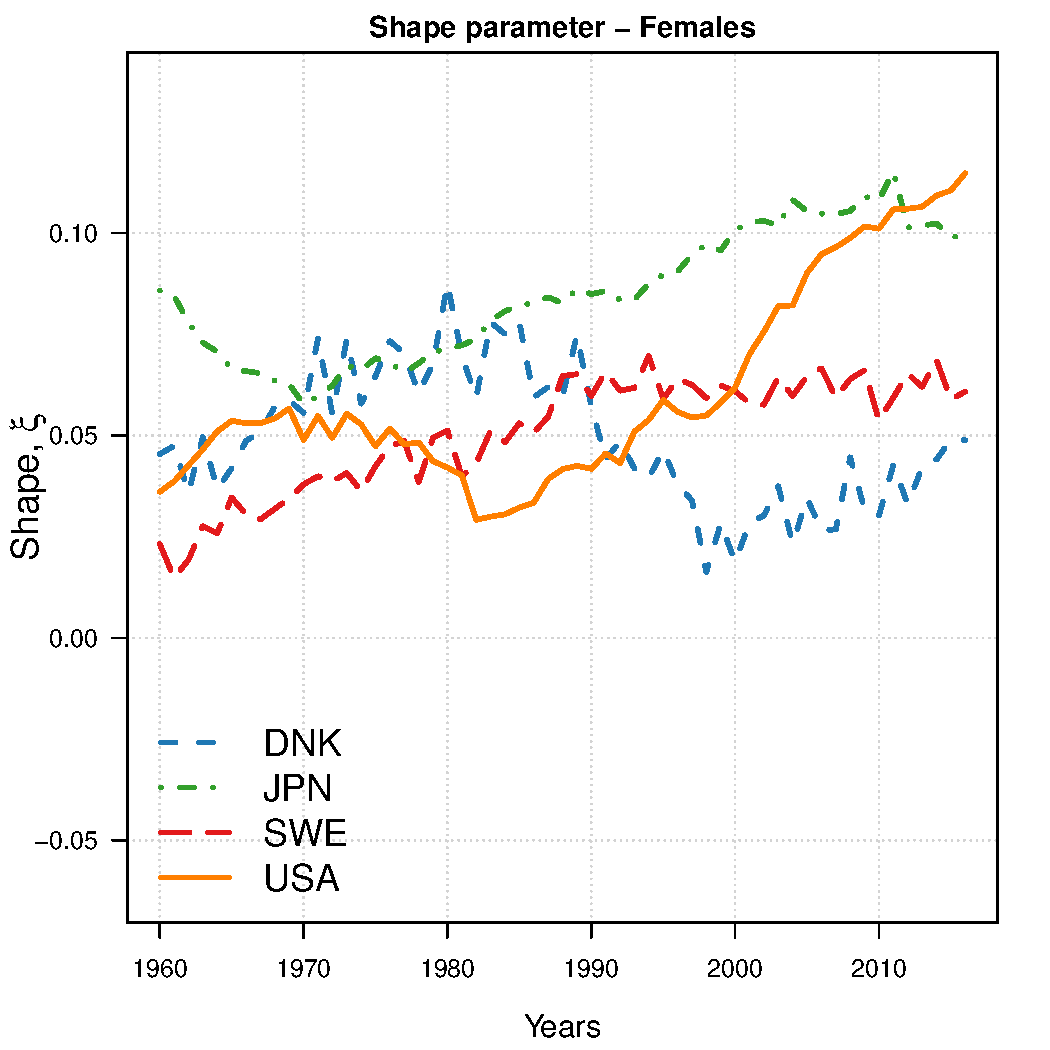
\includegraphics[scale=.4]{./Ch2/F9a.pdf}
	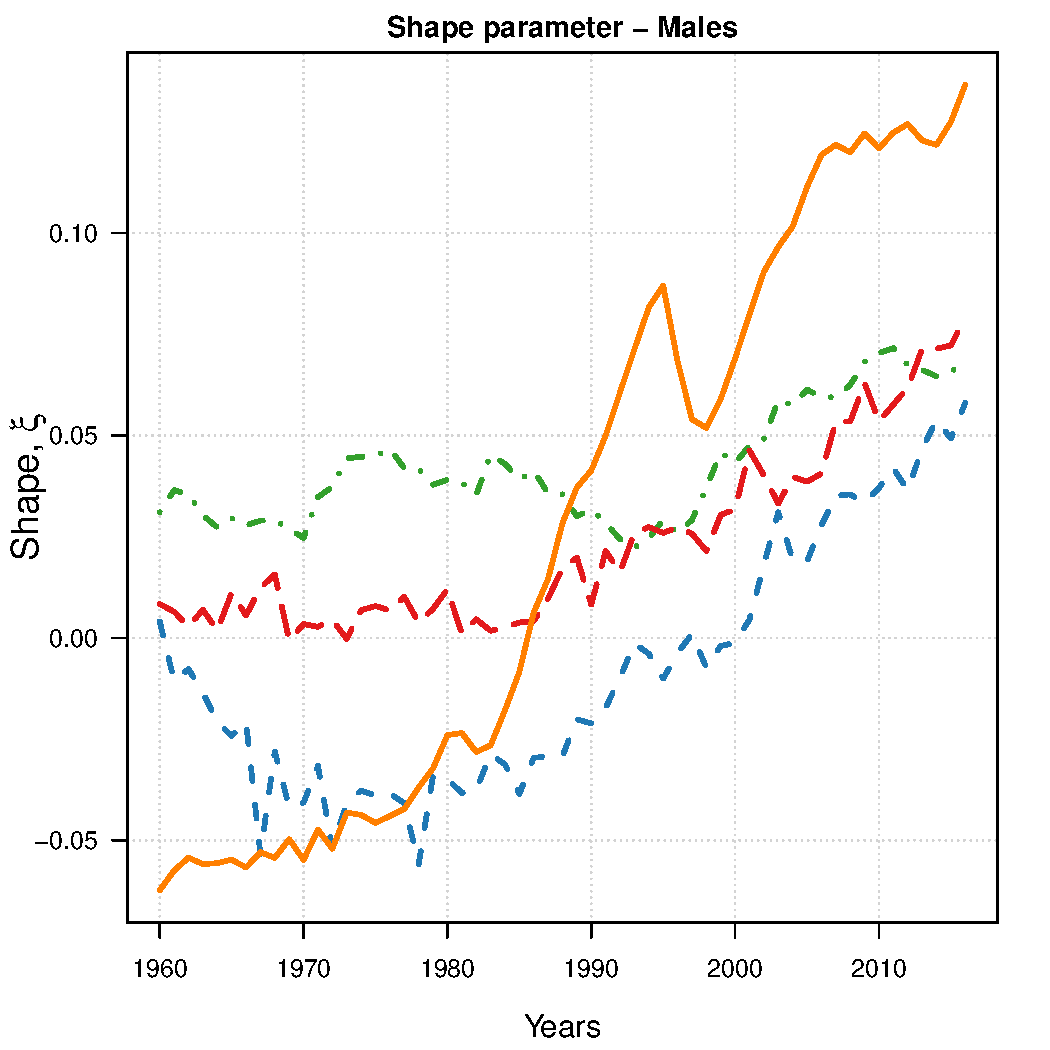
\includegraphics[scale=.4]{./Ch2/F9b.pdf}
	
	\caption{Estimated shape $\xi$ parameters of the Minimal Generalized Extreme-Value model for female (left) and male (right panel) adults aged 30-110+ in four high-longevity countries during 1960-2016.}\label{Fig:ShapeParam}
	
	
\end{figure}

Figure~\ref{Fig:Dx2016EV} shows the estimated MinGEV age-at-death distributions for the four countries by sex in 2016. From the Figure, it is possible to observe that the share of premature deaths for USA females and males is higher than for the other three countries. In addition, the smaller compression of the USA distribution of deaths compared to the other countries clearly emerges from the two graphs.

\begin{figure}[!ht]
	\begin{center}
		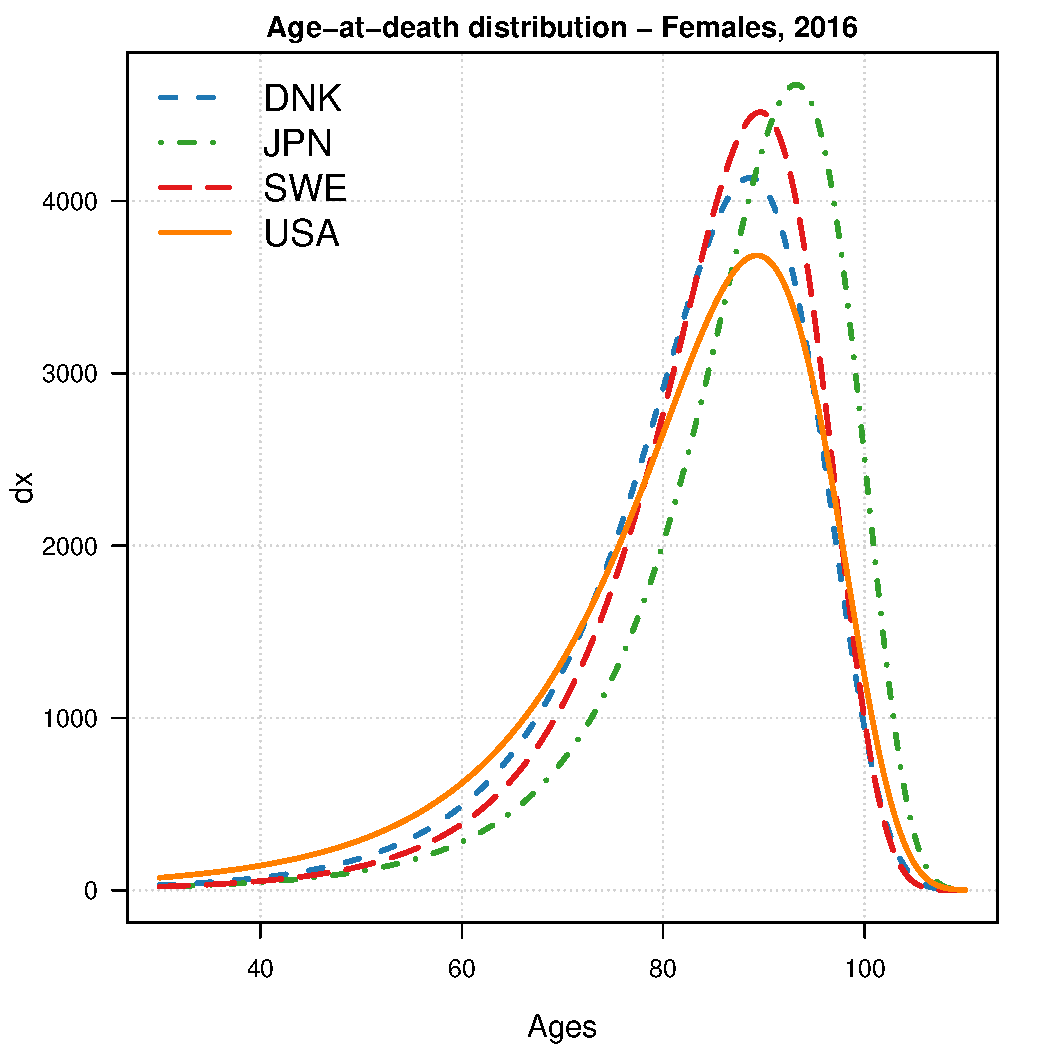
\includegraphics[scale=0.4]{./Ch2/F10a.pdf}
		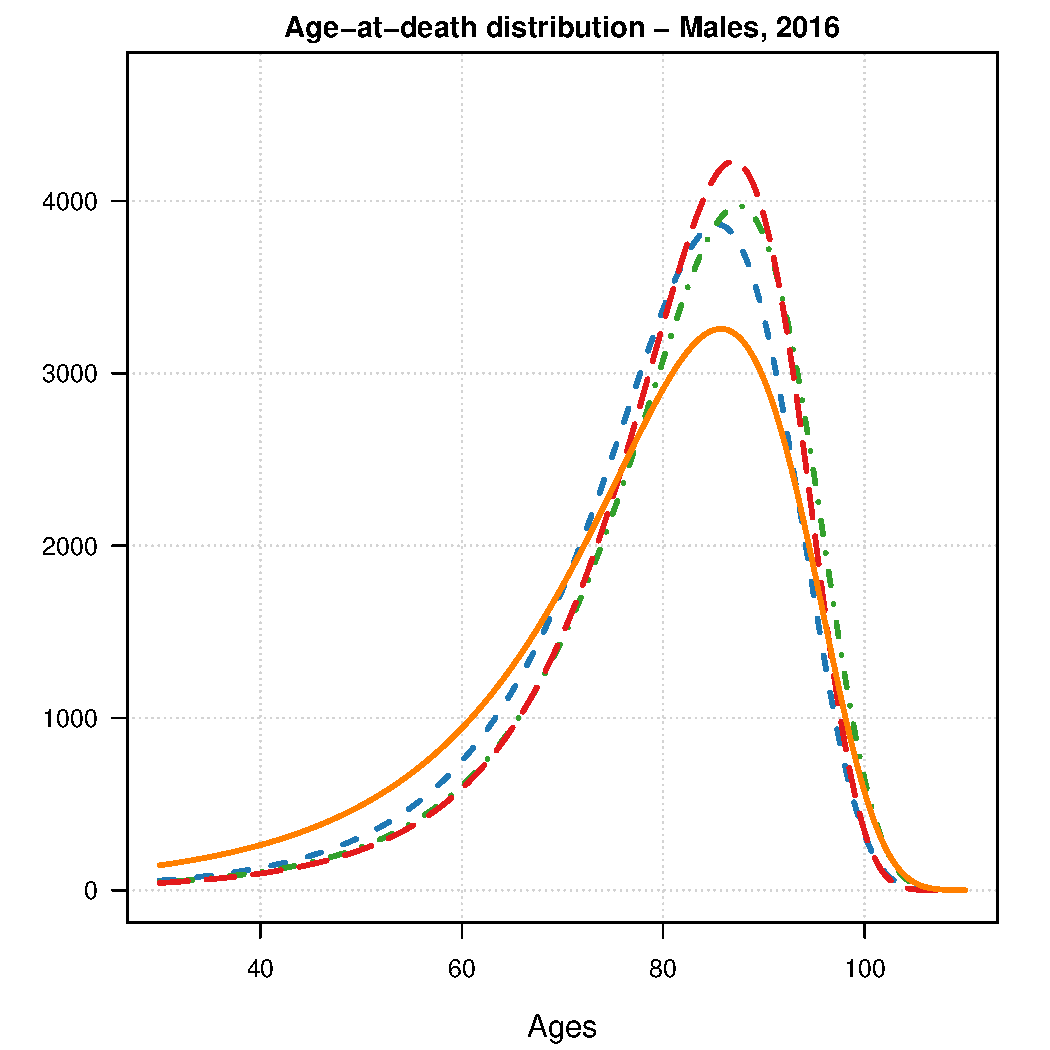
\includegraphics[scale=0.4]{./Ch2/F10b.pdf} 		
		\caption{Age-at-death distributions in 2016 for female (left) and male (right panel) adults aged 30-110+ in four high-longevity countries corresponding to the Minimal Generalized Extreme-Value model estimates.}\label{Fig:Dx2016EV}
		
	\end{center}  
\end{figure}

Figure~\ref{Fig:Ch2LocSca6models} shows the location $u$ and scale $c$ estimates for six models of the LS family fitted to Swedish adult female and male mortality during 1960-2016. The parameters have been rescaled for comparability, and while here we focus on Sweden, the results are the same for the other countries.

\begin{figure}[!ht]
	\begin{center}
		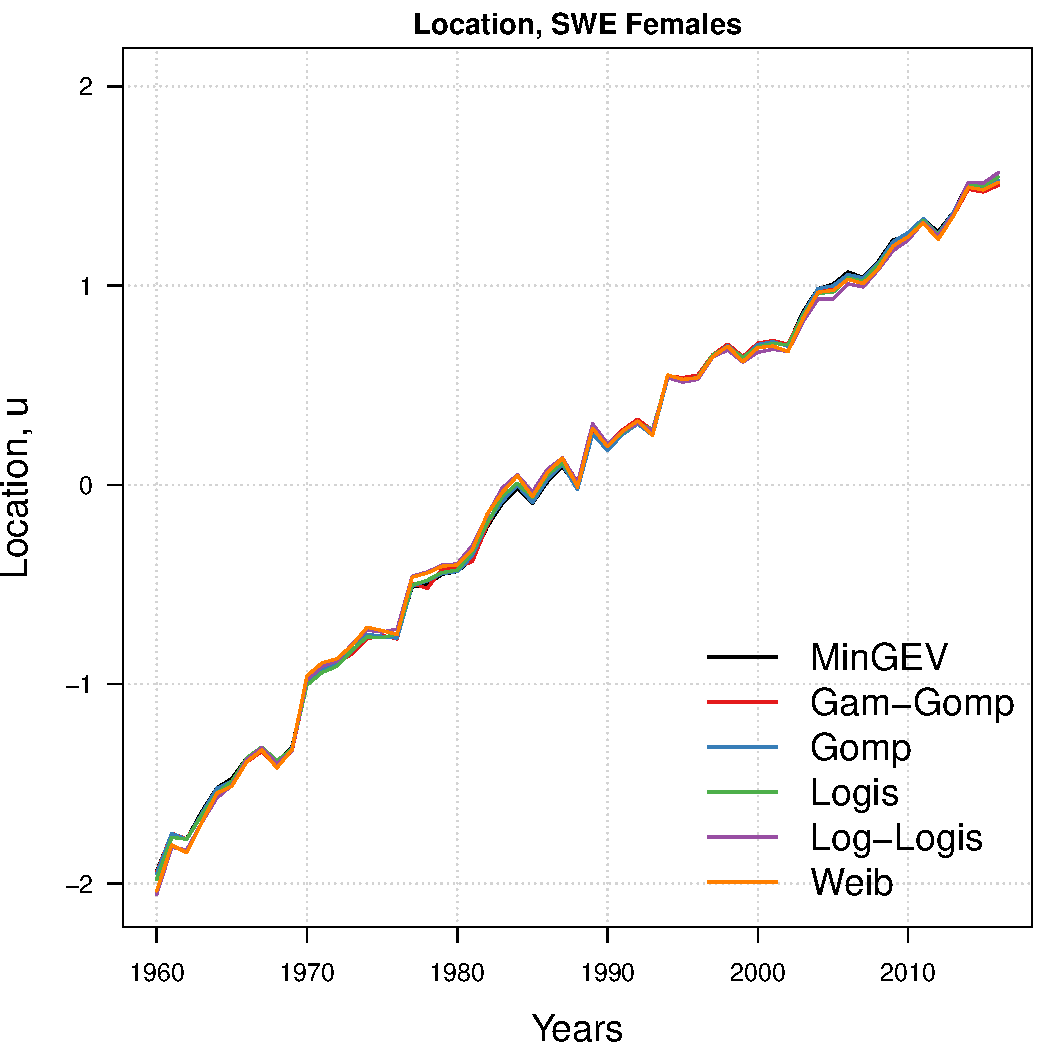
\includegraphics[scale=0.4]{./Ch2/F11a.pdf}
		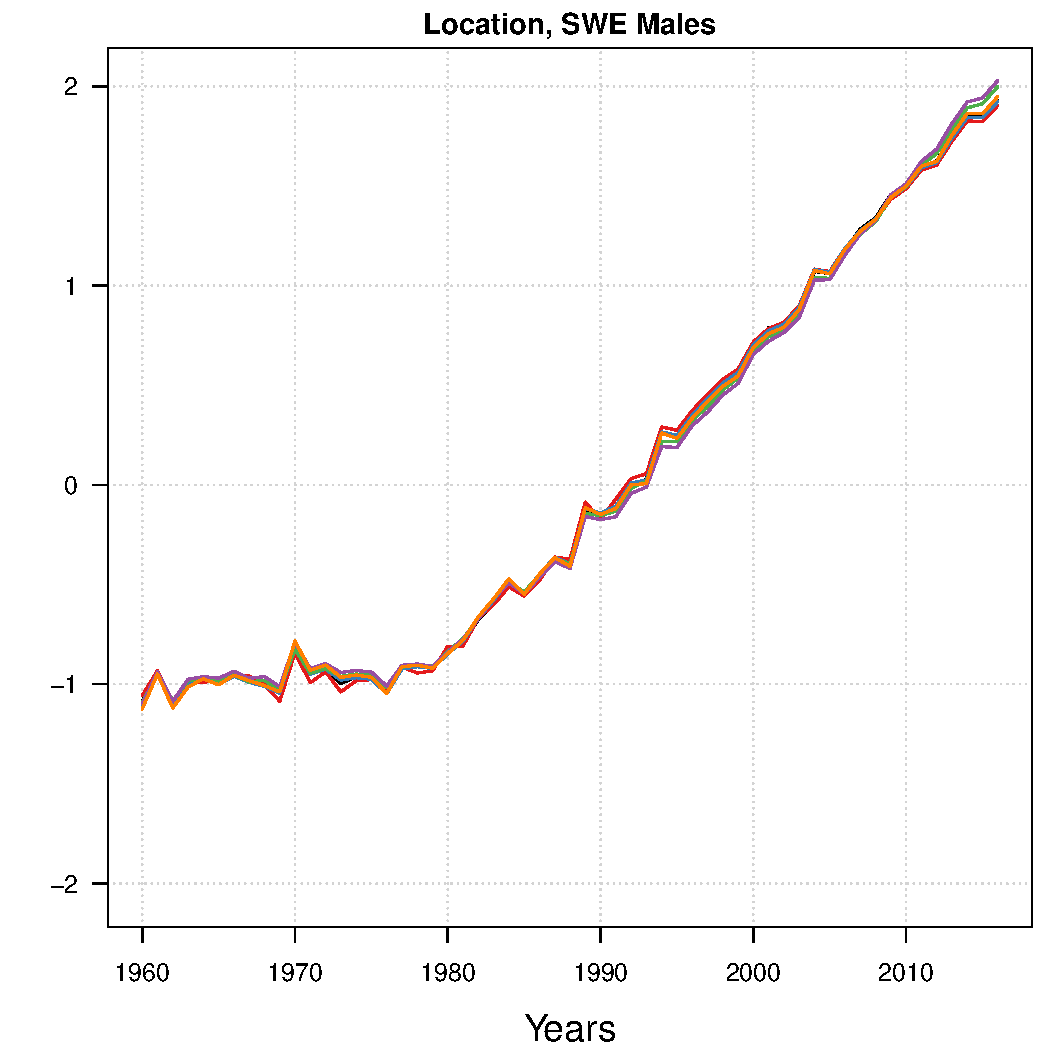
\includegraphics[scale=0.4]{./Ch2/F11b.pdf} 
		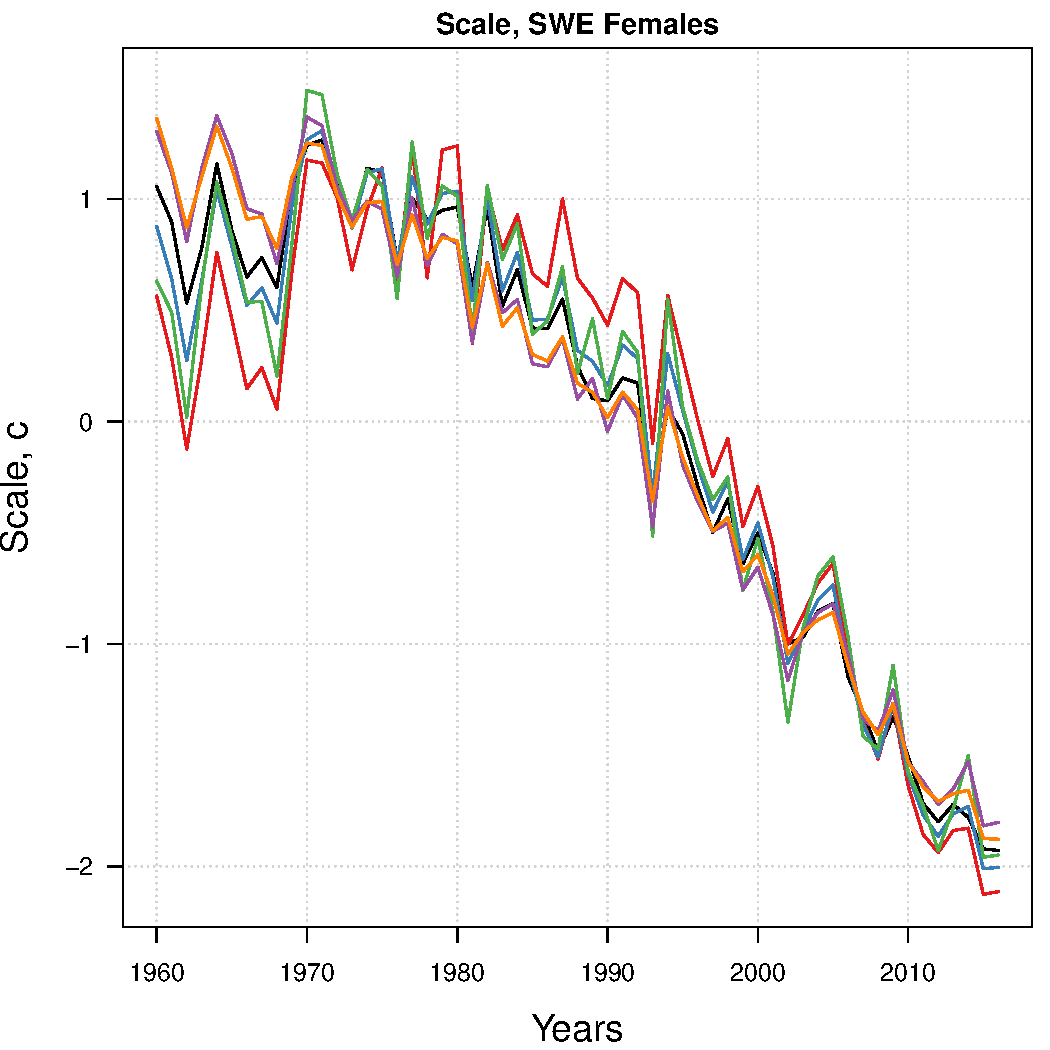
\includegraphics[scale=0.4]{./Ch2/F11c.pdf}
		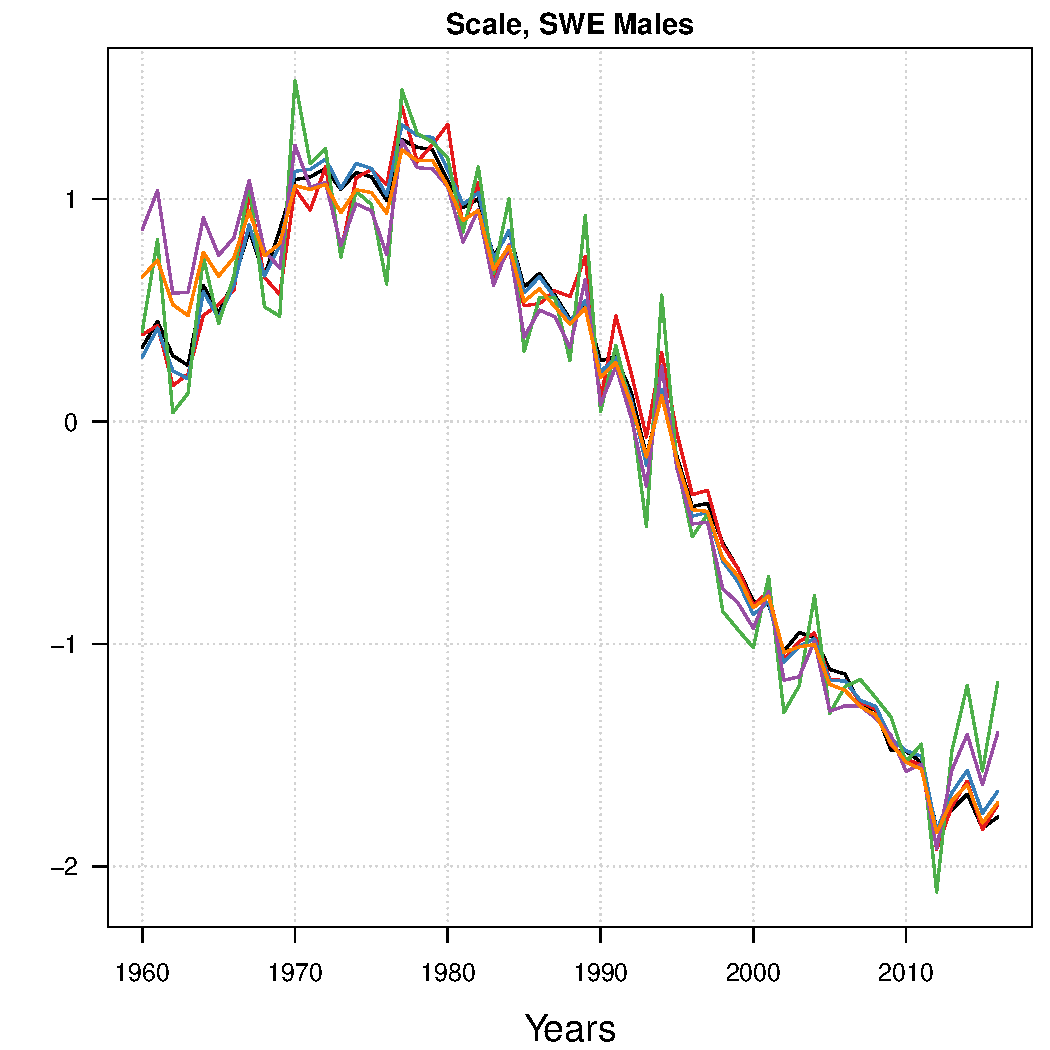
\includegraphics[scale=0.4]{./Ch2/F11d.pdf}
		
		\caption{Location $u$ and scale $c$ rescaled estimates of six LS models for female and male adults aged 30-110+ in Sweden during 1960-2016.\label{Fig:Ch2LocSca6models}} 
		
	\end{center}  
\end{figure}

The Figure shows that the location and scale estimates are very consistent across models: the former are always extremely close to each other, as well as the latter which are characterized by a slightly higher volatility. As such, the very same patterns of shifting and compression dynamics emerge from employing different LS models due to the similarity of the models' estimates.


\subsection{Decomposition of mortality changes into location and scale effects}\label{Subsec:Ch2appE}

Here, we decompose changes in life expectancy at age 30 ($\dot{e}_{30,t}$) into two components:
\begin{equation}\label{Eq:DecomposeE30}
\dot{e}_{30,t} = \Delta u + \Delta c \, ,
\end{equation}
where $\Delta u$ and $\Delta c$ are the gains in life expectancy resulting from the changes in the location (shift) and scale (compression) parameters, respectively.

Taking advantage of the findings reported in Fig.~\ref{Fig:Ch2LocSca6models}, namely the consistency and comparability of the location--scale parameters across different specification of the LS family, we focus on the decomposition of the Gompertz model. Specifically, we extend the methodology presented by \cite{bergeron2015decomposing} to the LS-like parameterization of the Gompertz model.

Equation~(\ref{GompertzMuLS}) introduced the LS-like parameterization of the Gompertz model. Here, we make explicit the time dependency of the model by letting the location and scale parameters be a function of time $t$:
\begin{eqnarray}\label{Eq:GompertzMuLSt}
\mu_{x,t} = \frac{1}{c_t} \, e^{\frac{x-u_t}{c_t}} \, .
\end{eqnarray}
Let a dot on top of a variable denote its derivative with respect to time \citep{vaupel2003decomposing}. The change over time in the force of mortality ($\dot{\mu}_{x,t}$) can be decomposed
into respective components of change for the location ($\dot{u}_{t}$) and scale ($\dot{c}_{t}$) parameters:
\begin{eqnarray}\label{Eq:ChangeGompertzLS}
\dot{\mu}_{x,t} &=& \dot{u}_{t} \left[ - \frac{\mu_{x,t}}{c_t} \right] + \dot{c}_{t} \left[ - \frac{\mu_{x,t}}{c_t} \left(1 + \frac{x-u_t}{c_t}\right) \right] \notag \\
&=& \dot{u}_{t} \, f_u(\mu_{x,t}) +  \dot{c}_{t} \, f_c(\mu_{x,t}) \, ,
\end{eqnarray}
where $f_u(\mu_{x,t})$ and $f_c(\mu_{x,t})$ are weighting function of the hazard rate for the location and scale parameters, respectively. 

Similarly to the force of mortality, we can derive the time change of life expectancy. Specifically, life expectancy at age 30 can be expressed as:
\begin{eqnarray}\label{Eq:E30}
e_{30,t} = \int_{30}^{\omega} l_{a,t} \, d_a \, ,
\end{eqnarray}
where $l_{a,t}$ is the survival function at age $a$ and time $t$. Changes in life expectancy at age 30 ($\dot{e}_{30,t}$) can thus be written as:
\begin{eqnarray}\label{Eq:E30overTime}
\dot{e}_{30,t} = \int_{30}^{\omega} \dot{l}_{a,t} \, d_a = - \int_{30}^{w} l_{a,t} \int_{30}^{a} \dot{\mu}_{x,t} \, d_x \, d_a \, ,
\end{eqnarray}
where $\dot{l}_{a,t}$ is the time derivative of the survival function. If we substitute Eq.~(\ref{Eq:ChangeGompertzLS}) into Eq.~(\ref{Eq:E30overTime}), we can decompose the changes in life expectancy at age 30 ($\dot{e}_{30,t}$) into changes due to the location and scale parameters as:
\begin{eqnarray}\label{Eq:ChangeE30GompertzLS}
\dot{e}_{30,t} = \underbrace{\dot{u}_{t} \int_{30}^{\omega} l_{a,t} \int_{30}^{a} f_u(\mu_{x,t}) \, d_x \, d_a}_\text{$\Delta u$} \, + \, \underbrace{\dot{c}_{t} \int_{30}^{w} l_{a,t} \int_{30}^{a} f_c(\mu_{x,t}) \, d_x \, d_a}_\text{$\Delta c$} \, .
\end{eqnarray}
The first term in Eq.~(\ref{Eq:ChangeE30GompertzLS}) represents the gain in life expectancy resulting from a
change in location ($\Delta u$), corresponding to a shifting pattern, while the second
term is the gain in life expectancy produced by a change in variability ($\Delta c$),
indicating a compression pattern. These are the equivalent terms of Eq.~(\ref{Eq:DecomposeE30}) in the Gompertz model. 
Specifically, we employ discrete approximations to estimate derivatives such as those in Eq.~(\ref{Eq:ChangeE30GompertzLS}) \cite[see][Appendix B]{bergeron2015decomposing}.

\cleardoublepage

\end{document}	